\documentclass{article} % For LaTeX2e
\usepackage{iclr2019_conference,times}

% Optional math commands from https://github.com/goodfeli/dlbook_notation.
%%%%% NEW MATH DEFINITIONS %%%%%

\usepackage{amsmath,amsfonts,bm}

% Mark sections of captions for referring to divisions of figures
\newcommand{\figleft}{{\em (Left)}}
\newcommand{\figcenter}{{\em (Center)}}
\newcommand{\figright}{{\em (Right)}}
\newcommand{\figtop}{{\em (Top)}}
\newcommand{\figbottom}{{\em (Bottom)}}
\newcommand{\captiona}{{\em (a)}}
\newcommand{\captionb}{{\em (b)}}
\newcommand{\captionc}{{\em (c)}}
\newcommand{\captiond}{{\em (d)}}

% Highlight a newly defined term
\newcommand{\newterm}[1]{{\bf #1}}


% Figure reference, lower-case.
\def\figref#1{figure~\ref{#1}}
% Figure reference, capital. For start of sentence
\def\Figref#1{Figure~\ref{#1}}
\def\twofigref#1#2{figures \ref{#1} and \ref{#2}}
\def\quadfigref#1#2#3#4{figures \ref{#1}, \ref{#2}, \ref{#3} and \ref{#4}}
% Section reference, lower-case.
\def\secref#1{section~\ref{#1}}
% Section reference, capital.
\def\Secref#1{Section~\ref{#1}}
% Reference to two sections.
\def\twosecrefs#1#2{sections \ref{#1} and \ref{#2}}
% Reference to three sections.
\def\secrefs#1#2#3{sections \ref{#1}, \ref{#2} and \ref{#3}}
% Reference to an equation, lower-case.
\def\eqref#1{Eq.~(\ref{#1})}
% Reference to an equation, upper case
\def\Eqref#1{Equation~\ref{#1}}
% A raw reference to an equation---avoid using if possible
\def\plaineqref#1{\ref{#1}}
% Reference to a chapter, lower-case.
\def\chapref#1{chapter~\ref{#1}}
% Reference to an equation, upper case.
\def\Chapref#1{Chapter~\ref{#1}}
% Reference to a range of chapters
\def\rangechapref#1#2{chapters\ref{#1}--\ref{#2}}
% Reference to an algorithm, lower-case.
\def\algref#1{algorithm~\ref{#1}}
% Reference to an algorithm, upper case.
\def\Algref#1{Algorithm~\ref{#1}}
\def\twoalgref#1#2{algorithms \ref{#1} and \ref{#2}}
\def\Twoalgref#1#2{Algorithms \ref{#1} and \ref{#2}}
% Reference to a part, lower case
\def\partref#1{part~\ref{#1}}
% Reference to a part, upper case
\def\Partref#1{Part~\ref{#1}}
\def\twopartref#1#2{parts \ref{#1} and \ref{#2}}

\def\ceil#1{\lceil #1 \rceil}
\def\floor#1{\lfloor #1 \rfloor}
\def\1{\bm{1}}
\newcommand{\train}{\mathcal{D}}
\newcommand{\valid}{\mathcal{D_{\mathrm{valid}}}}
\newcommand{\test}{\mathcal{D_{\mathrm{test}}}}

\def\eps{{\epsilon}}


% Random variables
\def\reta{{\textnormal{$\eta$}}}
\def\ra{{\textnormal{a}}}
\def\rb{{\textnormal{b}}}
\def\rc{{\textnormal{c}}}
\def\rd{{\textnormal{d}}}
\def\re{{\textnormal{e}}}
\def\rf{{\textnormal{f}}}
\def\rg{{\textnormal{g}}}
\def\rh{{\textnormal{h}}}
\def\ri{{\textnormal{i}}}
\def\rj{{\textnormal{j}}}
\def\rk{{\textnormal{k}}}
\def\rl{{\textnormal{l}}}
% rm is already a command, just don't name any random variables m
\def\rn{{\textnormal{n}}}
\def\ro{{\textnormal{o}}}
\def\rp{{\textnormal{p}}}
\def\rq{{\textnormal{q}}}
\def\rr{{\textnormal{r}}}
\def\rs{{\textnormal{s}}}
\def\rt{{\textnormal{t}}}
\def\ru{{\textnormal{u}}}
\def\rv{{\textnormal{v}}}
\def\rw{{\textnormal{w}}}
\def\rx{{\textnormal{x}}}
\def\ry{{\textnormal{y}}}
\def\rz{{\textnormal{z}}}

% Random vectors
\def\rvepsilon{{\mathbf{\epsilon}}}
\def\rvtheta{{\mathbf{\theta}}}
\def\rva{{\mathbf{a}}}
\def\rvb{{\mathbf{b}}}
\def\rvc{{\mathbf{c}}}
\def\rvd{{\mathbf{d}}}
\def\rve{{\mathbf{e}}}
\def\rvf{{\mathbf{f}}}
\def\rvg{{\mathbf{g}}}
\def\rvh{{\mathbf{h}}}
\def\rvu{{\mathbf{i}}}
\def\rvj{{\mathbf{j}}}
\def\rvk{{\mathbf{k}}}
\def\rvl{{\mathbf{l}}}
\def\rvm{{\mathbf{m}}}
\def\rvn{{\mathbf{n}}}
\def\rvo{{\mathbf{o}}}
\def\rvp{{\mathbf{p}}}
\def\rvq{{\mathbf{q}}}
\def\rvr{{\mathbf{r}}}
\def\rvs{{\mathbf{s}}}
\def\rvt{{\mathbf{t}}}
\def\rvu{{\mathbf{u}}}
\def\rvv{{\mathbf{v}}}
\def\rvw{{\mathbf{w}}}
\def\rvx{{\mathbf{x}}}
\def\rvy{{\mathbf{y}}}
\def\rvz{{\mathbf{z}}}

% Elements of random vectors
\def\erva{{\textnormal{a}}}
\def\ervb{{\textnormal{b}}}
\def\ervc{{\textnormal{c}}}
\def\ervd{{\textnormal{d}}}
\def\erve{{\textnormal{e}}}
\def\ervf{{\textnormal{f}}}
\def\ervg{{\textnormal{g}}}
\def\ervh{{\textnormal{h}}}
\def\ervi{{\textnormal{i}}}
\def\ervj{{\textnormal{j}}}
\def\ervk{{\textnormal{k}}}
\def\ervl{{\textnormal{l}}}
\def\ervm{{\textnormal{m}}}
\def\ervn{{\textnormal{n}}}
\def\ervo{{\textnormal{o}}}
\def\ervp{{\textnormal{p}}}
\def\ervq{{\textnormal{q}}}
\def\ervr{{\textnormal{r}}}
\def\ervs{{\textnormal{s}}}
\def\ervt{{\textnormal{t}}}
\def\ervu{{\textnormal{u}}}
\def\ervv{{\textnormal{v}}}
\def\ervw{{\textnormal{w}}}
\def\ervx{{\textnormal{x}}}
\def\ervy{{\textnormal{y}}}
\def\ervz{{\textnormal{z}}}

% Random matrices
\def\rmA{{\mathbf{A}}}
\def\rmB{{\mathbf{B}}}
\def\rmC{{\mathbf{C}}}
\def\rmD{{\mathbf{D}}}
\def\rmE{{\mathbf{E}}}
\def\rmF{{\mathbf{F}}}
\def\rmG{{\mathbf{G}}}
\def\rmH{{\mathbf{H}}}
\def\rmI{{\mathbf{I}}}
\def\rmJ{{\mathbf{J}}}
\def\rmK{{\mathbf{K}}}
\def\rmL{{\mathbf{L}}}
\def\rmM{{\mathbf{M}}}
\def\rmN{{\mathbf{N}}}
\def\rmO{{\mathbf{O}}}
\def\rmP{{\mathbf{P}}}
\def\rmQ{{\mathbf{Q}}}
\def\rmR{{\mathbf{R}}}
\def\rmS{{\mathbf{S}}}
\def\rmT{{\mathbf{T}}}
\def\rmU{{\mathbf{U}}}
\def\rmV{{\mathbf{V}}}
\def\rmW{{\mathbf{W}}}
\def\rmX{{\mathbf{X}}}
\def\rmY{{\mathbf{Y}}}
\def\rmZ{{\mathbf{Z}}}

% Elements of random matrices
\def\ermA{{\textnormal{A}}}
\def\ermB{{\textnormal{B}}}
\def\ermC{{\textnormal{C}}}
\def\ermD{{\textnormal{D}}}
\def\ermE{{\textnormal{E}}}
\def\ermF{{\textnormal{F}}}
\def\ermG{{\textnormal{G}}}
\def\ermH{{\textnormal{H}}}
\def\ermI{{\textnormal{I}}}
\def\ermJ{{\textnormal{J}}}
\def\ermK{{\textnormal{K}}}
\def\ermL{{\textnormal{L}}}
\def\ermM{{\textnormal{M}}}
\def\ermN{{\textnormal{N}}}
\def\ermO{{\textnormal{O}}}
\def\ermP{{\textnormal{P}}}
\def\ermQ{{\textnormal{Q}}}
\def\ermR{{\textnormal{R}}}
\def\ermS{{\textnormal{S}}}
\def\ermT{{\textnormal{T}}}
\def\ermU{{\textnormal{U}}}
\def\ermV{{\textnormal{V}}}
\def\ermW{{\textnormal{W}}}
\def\ermX{{\textnormal{X}}}
\def\ermY{{\textnormal{Y}}}
\def\ermZ{{\textnormal{Z}}}

% Vectors
\def\vzero{{\bm{0}}}
\def\vone{{\bm{1}}}
\def\vmu{{\bm{\mu}}}
\def\vtheta{{\bm{\theta}}}
\def\va{{\bm{a}}}
\def\vb{{\bm{b}}}
\def\vc{{\bm{c}}}
\def\vd{{\bm{d}}}
\def\ve{{\bm{e}}}
\def\vf{{\bm{f}}}
\def\vg{{\bm{g}}}
\def\vh{{\bm{h}}}
\def\vi{{\bm{i}}}
\def\vj{{\bm{j}}}
\def\vk{{\bm{k}}}
\def\vl{{\bm{l}}}
\def\vm{{\bm{m}}}
\def\vn{{\bm{n}}}
\def\vo{{\bm{o}}}
\def\vp{{\bm{p}}}
\def\vq{{\bm{q}}}
\def\vr{{\bm{r}}}
\def\vs{{\bm{s}}}
\def\vt{{\bm{t}}}
\def\vu{{\bm{u}}}
\def\vv{{\bm{v}}}
\def\vw{{\bm{w}}}
\def\vx{{\bm{x}}}
\def\vy{{\bm{y}}}
\def\vz{{\bm{z}}}

% Elements of vectors
\def\evalpha{{\alpha}}
\def\evbeta{{\beta}}
\def\evepsilon{{\epsilon}}
\def\evlambda{{\lambda}}
\def\evomega{{\omega}}
\def\evmu{{\mu}}
\def\evpsi{{\psi}}
\def\evsigma{{\sigma}}
\def\evtheta{{\theta}}
\def\eva{{a}}
\def\evb{{b}}
\def\evc{{c}}
\def\evd{{d}}
\def\eve{{e}}
\def\evf{{f}}
\def\evg{{g}}
\def\evh{{h}}
\def\evi{{i}}
\def\evj{{j}}
\def\evk{{k}}
\def\evl{{l}}
\def\evm{{m}}
\def\evn{{n}}
\def\evo{{o}}
\def\evp{{p}}
\def\evq{{q}}
\def\evr{{r}}
\def\evs{{s}}
\def\evt{{t}}
\def\evu{{u}}
\def\evv{{v}}
\def\evw{{w}}
\def\evx{{x}}
\def\evy{{y}}
\def\evz{{z}}

% Matrix
\def\mA{{\bm{A}}}
\def\mB{{\bm{B}}}
\def\mC{{\bm{C}}}
\def\mD{{\bm{D}}}
\def\mE{{\bm{E}}}
\def\mF{{\bm{F}}}
\def\mG{{\bm{G}}}
\def\mH{{\bm{H}}}
\def\mI{{\bm{I}}}
\def\mJ{{\bm{J}}}
\def\mK{{\bm{K}}}
\def\mL{{\bm{L}}}
\def\mM{{\bm{M}}}
\def\mN{{\bm{N}}}
\def\mO{{\bm{O}}}
\def\mP{{\bm{P}}}
\def\mQ{{\bm{Q}}}
\def\mR{{\bm{R}}}
\def\mS{{\bm{S}}}
\def\mT{{\bm{T}}}
\def\mU{{\bm{U}}}
\def\mV{{\bm{V}}}
\def\mW{{\bm{W}}}
\def\mX{{\bm{X}}}
\def\mY{{\bm{Y}}}
\def\mZ{{\bm{Z}}}
\def\mBeta{{\bm{\beta}}}
\def\mPhi{{\bm{\Phi}}}
\def\mLambda{{\bm{\Lambda}}}
\def\mSigma{{\bm{\Sigma}}}

% Tensor
\DeclareMathAlphabet{\mathsfit}{\encodingdefault}{\sfdefault}{m}{sl}
\SetMathAlphabet{\mathsfit}{bold}{\encodingdefault}{\sfdefault}{bx}{n}
\newcommand{\tens}[1]{\bm{\mathsfit{#1}}}
\def\tA{{\tens{A}}}
\def\tB{{\tens{B}}}
\def\tC{{\tens{C}}}
\def\tD{{\tens{D}}}
\def\tE{{\tens{E}}}
\def\tF{{\tens{F}}}
\def\tG{{\tens{G}}}
\def\tH{{\tens{H}}}
\def\tI{{\tens{I}}}
\def\tJ{{\tens{J}}}
\def\tK{{\tens{K}}}
\def\tL{{\tens{L}}}
\def\tM{{\tens{M}}}
\def\tN{{\tens{N}}}
\def\tO{{\tens{O}}}
\def\tP{{\tens{P}}}
\def\tQ{{\tens{Q}}}
\def\tR{{\tens{R}}}
\def\tS{{\tens{S}}}
\def\tT{{\tens{T}}}
\def\tU{{\tens{U}}}
\def\tV{{\tens{V}}}
\def\tW{{\tens{W}}}
\def\tX{{\tens{X}}}
\def\tY{{\tens{Y}}}
\def\tZ{{\tens{Z}}}


% Graph
\def\gA{{\mathcal{A}}}
\def\gB{{\mathcal{B}}}
\def\gC{{\mathcal{C}}}
\def\gD{{\mathcal{D}}}
\def\gE{{\mathcal{E}}}
\def\gF{{\mathcal{F}}}
\def\gG{{\mathcal{G}}}
\def\gH{{\mathcal{H}}}
\def\gI{{\mathcal{I}}}
\def\gJ{{\mathcal{J}}}
\def\gK{{\mathcal{K}}}
\def\gL{{\mathcal{L}}}
\def\gM{{\mathcal{M}}}
\def\gN{{\mathcal{N}}}
\def\gO{{\mathcal{O}}}
\def\gP{{\mathcal{P}}}
\def\gQ{{\mathcal{Q}}}
\def\gR{{\mathcal{R}}}
\def\gS{{\mathcal{S}}}
\def\gT{{\mathcal{T}}}
\def\gU{{\mathcal{U}}}
\def\gV{{\mathcal{V}}}
\def\gW{{\mathcal{W}}}
\def\gX{{\mathcal{X}}}
\def\gY{{\mathcal{Y}}}
\def\gZ{{\mathcal{Z}}}

% Sets
\def\sA{{\mathbb{A}}}
\def\sB{{\mathbb{B}}}
\def\sC{{\mathbb{C}}}
\def\sD{{\mathbb{D}}}
% Don't use a set called E, because this would be the same as our symbol
% for expectation.
\def\sF{{\mathbb{F}}}
\def\sG{{\mathbb{G}}}
\def\sH{{\mathbb{H}}}
\def\sI{{\mathbb{I}}}
\def\sJ{{\mathbb{J}}}
\def\sK{{\mathbb{K}}}
\def\sL{{\mathbb{L}}}
\def\sM{{\mathbb{M}}}
\def\sN{{\mathbb{N}}}
\def\sO{{\mathbb{O}}}
\def\sP{{\mathbb{P}}}
\def\sQ{{\mathbb{Q}}}
\def\sR{{\mathbb{R}}}
\def\sS{{\mathbb{S}}}
\def\sT{{\mathbb{T}}}
\def\sU{{\mathbb{U}}}
\def\sV{{\mathbb{V}}}
\def\sW{{\mathbb{W}}}
\def\sX{{\mathbb{X}}}
\def\sY{{\mathbb{Y}}}
\def\sZ{{\mathbb{Z}}}

% Entries of a matrix
\def\emLambda{{\Lambda}}
\def\emA{{A}}
\def\emB{{B}}
\def\emC{{C}}
\def\emD{{D}}
\def\emE{{E}}
\def\emF{{F}}
\def\emG{{G}}
\def\emH{{H}}
\def\emI{{I}}
\def\emJ{{J}}
\def\emK{{K}}
\def\emL{{L}}
\def\emM{{M}}
\def\emN{{N}}
\def\emO{{O}}
\def\emP{{P}}
\def\emQ{{Q}}
\def\emR{{R}}
\def\emS{{S}}
\def\emT{{T}}
\def\emU{{U}}
\def\emV{{V}}
\def\emW{{W}}
\def\emX{{X}}
\def\emY{{Y}}
\def\emZ{{Z}}
\def\emSigma{{\Sigma}}

% entries of a tensor
% Same font as tensor, without \bm wrapper
\newcommand{\etens}[1]{\mathsfit{#1}}
\def\etLambda{{\etens{\Lambda}}}
\def\etA{{\etens{A}}}
\def\etB{{\etens{B}}}
\def\etC{{\etens{C}}}
\def\etD{{\etens{D}}}
\def\etE{{\etens{E}}}
\def\etF{{\etens{F}}}
\def\etG{{\etens{G}}}
\def\etH{{\etens{H}}}
\def\etI{{\etens{I}}}
\def\etJ{{\etens{J}}}
\def\etK{{\etens{K}}}
\def\etL{{\etens{L}}}
\def\etM{{\etens{M}}}
\def\etN{{\etens{N}}}
\def\etO{{\etens{O}}}
\def\etP{{\etens{P}}}
\def\etQ{{\etens{Q}}}
\def\etR{{\etens{R}}}
\def\etS{{\etens{S}}}
\def\etT{{\etens{T}}}
\def\etU{{\etens{U}}}
\def\etV{{\etens{V}}}
\def\etW{{\etens{W}}}
\def\etX{{\etens{X}}}
\def\etY{{\etens{Y}}}
\def\etZ{{\etens{Z}}}

% The true underlying data generating distribution
\newcommand{\pdata}{p_{\rm{data}}}
% The empirical distribution defined by the training set
\newcommand{\ptrain}{\hat{p}_{\rm{data}}}
\newcommand{\Ptrain}{\hat{P}_{\rm{data}}}
% The model distribution
\newcommand{\pmodel}{p_{\rm{model}}}
\newcommand{\Pmodel}{P_{\rm{model}}}
\newcommand{\ptildemodel}{\tilde{p}_{\rm{model}}}
% Stochastic autoencoder distributions
\newcommand{\pencode}{p_{\rm{encoder}}}
\newcommand{\pdecode}{p_{\rm{decoder}}}
\newcommand{\precons}{p_{\rm{reconstruct}}}

\newcommand{\laplace}{\mathrm{Laplace}} % Laplace distribution

\newcommand{\E}{\mathbb{E}}
\newcommand{\Ls}{\mathcal{L}}
\newcommand{\R}{\mathbb{R}}
\newcommand{\emp}{\tilde{p}}
\newcommand{\lr}{\alpha}
\newcommand{\reg}{\lambda}
\newcommand{\rect}{\mathrm{rectifier}}
\newcommand{\softmax}{\mathrm{softmax}}
\newcommand{\sigmoid}{\sigma}
\newcommand{\softplus}{\zeta}
\newcommand{\KL}{D_{\mathrm{KL}}}
\newcommand{\Var}{\mathrm{Var}}
\newcommand{\standarderror}{\mathrm{SE}}
\newcommand{\Cov}{\mathrm{Cov}}
% Wolfram Mathworld says $L^2$ is for function spaces and $\ell^2$ is for vectors
% But then they seem to use $L^2$ for vectors throughout the site, and so does
% wikipedia.
\newcommand{\normlzero}{L^0}
\newcommand{\normlone}{L^1}
\newcommand{\normltwo}{L^2}
\newcommand{\normlp}{L^p}
\newcommand{\normmax}{L^\infty}

\newcommand{\parents}{Pa} % See usage in notation.tex. Chosen to match Daphne's book.

\DeclareMathOperator*{\argmax}{arg\,max}
\DeclareMathOperator*{\argmin}{arg\,min}

\DeclareMathOperator{\sign}{sign}
\DeclareMathOperator{\Tr}{Tr}
\let\ab\allowbreak

\usepackage{graphicx}
\usepackage{amsthm}
\usepackage{amssymb}
\usepackage{hyperref}
\usepackage{algorithm}
\usepackage{algpseudocode}
\usepackage{cleveref}
\usepackage{enumitem}
\usepackage{soul}
\usepackage{caption}
\usepackage{lipsum}
\usepackage{thmtools,thm-restate}
\newtheorem{lemma}{Lemma}
\crefname{lemma}{Lemma}{Lemmas}
\newcommand{\Le}[1]{{\color{red}{\bf\sf [ #1]}}}
\newcommand{\xc}[1]{{\color{blue}{\bf\sf [#1]}}}
\newcommand{\xinshi}[1]{{\color{black}{#1}}}
\newcommand{\shuang}[1]{{\color{purple}{\bf\sf[ #1]}}}
% \newcommand{\shuang}[1]{{\color{purple}{\bf\sf}}}
\newcommand{\Li}[1]{{\color{cyan}{\bf\sf [Li: #1]}}}


\graphicspath{{./Figs/}}



\title{Neural Model-Based Reinforcement Learning for Recommendation}

% Authors must not appear in the submitted version. They should be hidden
% as long as the \iclrfinalcopy macro remains commented out below.
% Non-anonymous submissions will be rejected without review.

\author{
XC, SL, other helpers, LS
\thanks{ Use footnote for providing further information
about author (webpage, alternative address)---\emph{not} for acknowledging
funding agencies.  Funding acknowledgements go at the end of the paper.} \\
Department of Computer Science\\
Cranberry-Lemon University\\
Pittsburgh, PA 15213, USA \\
\texttt{\{hippo,brain,jen\}@cs.cranberry-lemon.edu} \\
\And
Ji Q. Ren \& Yevgeny LeNet \\
Department of Computational Neuroscience \\
University of the Witwatersrand \\
Joburg, South Africa \\
\texttt{\{robot,net\}@wits.ac.za} \\
\AND
Coauthor \\
Affiliation \\
Address \\
\texttt{email}
}

% The \author macro works with any number of authors. There are two commands
% used to separate the names and addresses of multiple authors: \And and \AND.
%
% Using \And between authors leaves it to \LaTeX{} to determine where to break
% the lines. Using \AND forces a linebreak at that point. So, if \LaTeX{}
% puts 3 of 4 authors names on the first line, and the last on the second
% line, try using \AND instead of \And before the third author name.

\newcommand{\fix}{\marginpar{FIX}}
\newcommand{\new}{\marginpar{NEW}}

%\iclrfinalcopy % Uncomment for camera-ready version, but NOT for submission.
\begin{document}


\maketitle

\begin{abstract}
 There is a great interest in applying reinforcement learning (RL) to recommendation systems. However, in this setting, an online user is the environment; neither the reward function nor the environment dynamics is clearly defined, making the application of RL challenging. 
 In this paper, we propose a novel model-based reinforcement learning framework for recommendation systems, where we developed a generative adversarial network to imitate user behavior dynamics and learn her reward function. Using this user model as the simulation environment, we develop a novel DQN algorithm to obtain a combinatorial recommendation policy which can handle a large number of candidate items efficiently. 
%  \xinshi{in time linear in the number}. 
 In our experiments with real data, we show this generative adversarial user model can better explain user behavior than alternatives, and the RL policy based on this model can lead to better long turn reward for the user \xinshi{and higher click rate for the system.}
\end{abstract}
\vspace{-3mm}
\section{Introduction}
\vspace{-3mm}
        \setlength{\abovedisplayskip}{4pt}
        \setlength{\abovedisplayshortskip}{1pt}
        \setlength{\belowdisplayskip}{4pt}
        \setlength{\belowdisplayshortskip}{1pt}
        \setlength{\jot}{3pt}
        \setlength{\textfloatsep}{6pt}	

Recommendation systems have become a crucial part of almost all online service platforms. A typical interaction between the
system and its users is --- users are recommended a page of items
and provide feedback; and then the system recommends a new
page of items. A common way of building recommendation systems is to estimate a model which minimizes the discrepancy between the model prediction and the \emph{immediate} user response according to some loss function. In other words, these models do not explicitly take into account the long term user interest. \xinshi{However, user's interest can evolve over time based on what she observes, and the recommender's action may significantly influence such evolution. In some sense the recommender is guiding users' interest by displaying particular items and hidding the rest. Thus, a recommendation strategy which takes user's long term interest into account is more favorable. 
% We will design a recommendation policy which does not only focus on the current click through rate, but aims at engaging the users to interact with the system actively in a long run. 
} 

Reinforcement learning (RL) is a learning paradigm where a policy will be obtained to take actions in an environment so as to maximize the expected long term reward. In the recommendation system setting, the environment will correspond to the logged online user, the reward function will be the user's interest, and the policy will correspond to the recommendation policy. Although RL framework has been successfully applied to many game settings, such as Atari games~\citep{MniKavSilRusetal15} and GO~\citep{SilHuaMadGueetal16}, it met a few challenges in the recommendation system setting. 

First, a user's interest (reward function) driving her behavior is typically unknown, yet it is critically important for the use of reinforcement learning algorithms. Essentially, without the reward function, neither model-based nor model-free reinforcement learning algorithms can be used. Thus, in existing use of RL for recommendation systems, the reward functions are typically manually designed which may or may not reflect user's true interests~\citep{zhao2018deep,zheng2018drn}.

Second, model-free reinforcement learning typically requires lots of interactions with the environment in order to learn a good policy. This is impractical in the recommendation system setting. A logged online user will quickly abandon the service if the recommendation looks random and do not meet user's interests. Thus, to avoid the large sample complexity of the model-free approach, a model-based RL approach is more preferable.
In a related but a different setting where one wants to train a robot policy, recent work showed that model-based reinforcement learning is much more sample efficient~\citep{NagabandiKahn17, DeisenrothFox15, IgnasiPieter18}. However, these approaches can not be used in the recommendation setting, since a user behavior model typically consists of sequences of discrete choices under complex session context.   

To address the above challenges, we propose a novel model-based reinforcement learning framework for recommendation systems, where we first recover a user behavior model from historical data, and then optimize a policy in response to this model. Our technical innovations are:
\begin{enumerate}[nosep,nolistsep]
    \item We develop a generative adversarial network formulation to imitate user behavior dynamics and recover her reward function. These two components are estimated simultaneously via a joint mini-max optimization algorithm; 
    \item Using this model as the simulation environment, we develop a cascaded DQN algorithm to obtain a recommendation policy. The cascaded design of action-value function allows us to handle a large number of items with time complexity only linear in the number. 
\end{enumerate}
In our experiments with real data, we showed that this generative adversarial model has a better fit to user behavior in terms of held-out likelihood and click prediction. Since our model can take historical items clicked by the user into account, these results show the benefits of explicitly modeling the influence of history on user's interests, and imply the potential usefulness of reinforcement learning. Based on the learned user model and reward, we show that the estimated recommendation policy leads to better cumulative long term reward for the user. Furthermore, in the case of model mismatch, our model-based policy can also quickly adapt to the new dynamics with much few number of user interactions compared to model-free approaches.    

% \shuang{ from Lihong Li's KDD paper: A couple of sentences might be used to highlight the proposed model-based reinforcement learning recommendation system. First, our goal is not to make recommendations not based on an individual's preferences, but instead based on the anticipated long-term interest level of a broad group of users from a target community. Second, we try to predict rather than detect popularity. Unlike individual interests, community interest level is not often immediately clear; there is a time lag before the level of interest starts to take off. Here, the goal is for the recommendation system to identify and track new items... in real time -- attempting to identify hot updates before they before they become hot to keep the user at the leading edge. For training purposes, we can use community response measured at a time much later than the original post or publication. This problem is well-suited to the reinforcement paradigm, since the reward (the level of community uptake or positive response) is not immediately known, so the system needs to learn a mechanism for estimating future reactions. }\Le{This second part is probably more suitable for the introduction or framework part to justify why one wants to use RL as the framework.} 

% \Le{
% Rough flow below. Will work on it when I am up again: 

% There is a great interests in applying reinforcement learning algorithm to recommendation systems. 

% Supposedly reinforcement learning algorithms take into account longer term reward of the user. 

% However, the user utility function is unknown and the transition dynamic is unknown. 

% In a related but a different setting where one wants to train a robot policy, typically the reward is known but the transition is unknown. This is also a very challenging task. Recent results showed that model-based reinforcement learning lead to much better results. 

% Can we also use model based reinforcement learning to improve the recommendation based on reinforcement learning? 

% In this paper we explore a model based reinforcement learning framework for recommendation. We observed that user the following behavior: exploration and exploitation. Thus we model the user as a GAN, and learn the reward function for the user using a mini-max formulation. 

% Then we optimize a policy according to this learned user model using DQN with experience replay. 

% We find that this model has a better fit to user behavior in terms of likelihood and explaining user behavior than alternatives (logistic regression and ccf). Furthermore, the learned policy is also able to make recommendation which leads to better long term reward, compared to directly learn reinforcement learning policy from data. 

% }

% Improving the policy of displaying items to users is a core task for online marketing in web services, internet media platforms, and e-commerce platforms. 
% % It is crucial for precision marketing that a recommender system can understand users' interests, and personalized recommendation is provided to the user. It thus becomes indispensable to learn each user's preference and his choice behavior.
% Previously, plenty of predictive user models have been designed to exploit a wealth of data collected from previous user interaction with the platform. However, it is commonly assumed in these models that users choose what they like~\citep{RicDomRag07, GraepelCandela10}, and user's past experience and active exploration-exploitation are not explicitly taken into account. 

% We include the online user as an active agent in the system who makes choices by optimizing her own objective function. We consider the learning of such unknown object by observing her actions.

% We align the rewards of recommender with the objects of users so as to achieve a strategy which aims at satisfying the users and engaging the users in the system for a long run.

\vspace{-3mm}
\section{Related Work}
\vspace{-3mm}

Commonly used recommendation algorithms typically use simple user model. For instance, logistic regression based wide\&deep networks~\citep{ChengKocHarmsen16} basically assume an user choose each item independently; collaborative competitive filtering~\citep{YanLonSmoEtal11b} takes into account the context of an user's choice, but assume each pageview is independent from each other. 
Session-based RNN~\citep{HidKarBalTik16} improves upon previous approaches by modeling user's history, but this model does not recover user's reward function and can not be used subsequently for reinforcement learning. Contextual bandit based approaches, such as LinUCB~\citep{LiChuLanSch10}, can deal with adversarial user behaviors, but the reward is used and updated in a Bayesian framework, not directly usable by a reinforcement learning framework. 
% \xc{feel a bit strange for the linUCB description here..}. 
% In contrast, we will design a more realistic user model and learn 
% the corresponding reward function suitable for subsequent reinforcement learning task. 

% Recently, \cite{XiangyuLiangZhuoye18,zhao2018deep,zheng2018drn} used RL for recommender systems. However, their reward functions in these work are typically manually designed and are not learned jointly with the user dynamics model. In contrast, our framework will learn the optimal reward functions which can explain the corresponding user bebavior model. Such matching reward function and user model facilitate subsequent recommendation policy optimization based on reinforcement learning.  

% Focus on what's the difference during description. No model, hand-designed reward. 

\cite{XiangyuLiangZhuoye18,zhao2018deep,zheng2018drn} used model-free RL for recommender systems, which may require many user interactions and the reward function is manually designed. Model-based reinforcement learning has been commonly used in robotics applications, and resulted in much reduced (interaction) sample complexity to obtain good policy~\citep{DeisenrothFox15,NagabandiKahn17,IgnasiPieter18}. The advantage of model-based approach is that potentially large amount of off-policy data can be pooled and used to learn a good environment dynamics model, whereas model-free approach can only use expensive on-policy data for learning. However, previous model-based approach are typically designed based on physics or Gaussian processes, and not tailored for complex sequences of user behaviors. 

% In contrast, our model treat the user as an intelligent agent which can optimize its own rewards, and take actions to balance her own exploration and exploitation.  

\vspace{-3mm}
\section{Setting and Overview of the Approach}
\vspace{-3mm}

We assume a typical interaction setting between the recommendation system and its users be -- {\bf in each pageview, users are recommended a page of $k$ items and provide feedback by clicking on only one of these items; and then the system recommends a new page of $k$ items.}

Since reinforcement learning can explicitly take into account longer term rewards, it holds the promise to improve user's long term engagement with an online platform. In the reinforcement learning language, a recommendation system wants to learn a recommendation policy $\pi(\vs)$ such that the long term expected reward is maximized, i.e.
% \xc{I rewrite (1-6) to make the definitions in this paper consistent and accurate.. although it brings some complexity.. see whether it is clear enough? for the rest of this paper, notations are corrected according to the definitions here.}
{\small \begin{align}
    \pi^\ast = \argmax_{\pi(\vs^t,\gI^t)}~\E\left[\sum_{t=0}^{\infty} \gamma^t r(\vs^t, \gA^t, a^t)\right],~\text{where}~\vs^0\sim p^0,~\gA^t \sim \Li{\pi(s^{t})},~\vs^{t+1} \sim P(\cdot | \vs^t, \gA^t). 
    \label{eq:rl}
\end{align}}

\Li{$p^{0}$ is not defined? $\pi(s)$ and $\pi{s^{t}, \gI^{t}}$ here are two different functions? }

Below we will elaborate on several key aspects of the above RL framework as instantiated in recommendation system setting: \begin{enumerate}[nosep, nolistsep]
    \item {\bf Environment}: will correspond to a logged online user who can click on one of the $k$ items displayed by the recommendation system in each pageview (or interaction).
    \item {\bf State $\vs^t \in \gS$}: will correspond to an ordered sequence of user's historical clicks. %some summary statistic of the user's historical sequence of clicks.  
    \item {\bf Action $\gA^t \in {\gI \choose k}$}: will correspond to a subset of $k$ items chosen by the recommendation system from $\gI$ to display to the user. The notation ${\gI \choose k}$ means all subset of size $k$ of $\gI$.
    \item {\bf State Transition $P(\cdot|\vs^t,\gA^t):\gS \times {\gI \choose k} \mapsto \gP(\gS)$}: will correspond to a user behavior model which returns the transition probability for $\vs^{t+1}$ given previous state $\vs^t$ and displayed items $\gA^t$. It is equivalent to the distribution $\phi(\vs^t, \gA^t)$ over user's action defined in our user model, which will be introduced in section~\ref{sec:user_model}.
    \item {\bf Reward Function} $r(\vs^t,\gA^t, a^t):\gS  \times {\gI \choose k}\times \gI \mapsto \sR$: will correspond to user's reward or satisfaction in state $\vs^t$ and after making her choice $a^t\in \gA^t$ from the set displayed by the recommendation system. Here we assume that the reward to the recommendation system is the same as user's interests. Thus, a recommendation algorithm which optimizes its long term reward is designed to satisfy the user in a long run. %equivalent to optimize user's long term interests. 
    One can also include the online platform's benefit to the reward, but in this paper we will focus on user's satisfaction. 
    \item {\bf Policy $\pi(\vs^t, \gI^t):\gS\times 2^{\gI} \mapsto \gP({\gI \choose k})$}: will correspond to a recommendation algorithm which takes user's state $\vs^t$ and returns the probability distribution of a subset of $\gI^t$  to be displayed. Here we introduce the notation $\gI^t \subset{\gI}$ to represent available items at time $t$.  
\end{enumerate}
\xinshi{{\bf Remark.}} We note that in the above mapping, {\bf Environment, State and State Transition} are associated with the user, the {\bf Action and Policy} are associated with the recommendation system, and \xinshi{the {\bf Reward Function} is associated with both the recommendation system and the user.} 
% \st{ and Reward Function are associated with the user, while the  Action and Policy are associated with the recommendation system, and the recommendation system uses the same  Reward Function as the user.}
%
Here we use the notation $r(\vs^t, \gA^t, a^t)$ to emphasize the dependency of the reward on the recommendation action, since user can only choose from the display set. However, the value of the reward is actually determined by user's state and the clicked item once the item is in the display set. Thus, in section~\ref{sec:user_model} when we discuss on the user model, we simply denote $r(\vs^t, a^t)=r(\vs^t, \gA^t, a^t)$ and assume $a^t\in \gA^t$ is true. In fact, $r(\vs^t, \gA^t, a^t) =r(\vs^t, a^t)\cdot \1(a^t\in \gA^t) $. 

%
% $s^t\in \gS$ and $a^t \in \gA$ are the state of the environment and the action of the agent respectively. $r(s^t,a^t):\gS \times \gA \mapsto \sR$ is a reward function, and $P(\cdot|s^t,a^t): \gS \times \gA \mapsto \gP$ returns the transition probability of the environment, i.e., the probability of the next state $s^{t+1}$ given the previous state $s^t$ and action $a^t$. The policy $\pi(s):\gS \mapsto \gP$ is the probability of taking action $a$ given state $s$. 
%

When both the reward function and the state transition model are given, the optimal policy $\pi^\ast$ in~\eqref{eq:rl} can be estimated by repeated query to the model using algorithms such as Q-learning~\citep{Watkins89}. Thus, our first goal is to learn user's reward function. Furthermore, since model-based reinforcement learning is more sample efficient, we will also estimate a user behavior model associate with the reward function. Given both the reward function and state transition model, we can then use \Li{\st{an}a} RL algorithm to obtain a recommendation policy. 

% \st{
% When only the reward function is given, learning a policy in a model-free fashion is very expensive in the recommendation system setting. A logged online user will quickly abandon the service if the recommendation looks random and do not meet user’s interests.

% A critical challenge facing RL in the recommendation system setting is that the user's reward function is typically unknown. Yet, both model-based and model-free reinforcement learning algorithms require reward functions to start with. }\xc{removed. the conclusion of this part is moved to the above paragraph.}

% \shuang{The above two paragraphs seem to repeat the main ideas in third and fourth paragraphs in Intro}

More specifically, our solution consists of two major innovations. The first component is a generative adversarial network for the user behavior model and reward function. We will design a position weighted sequence model to embed the user's historical sequence of clicks into the user state $\vs^t$, and then use this state to define the reward function of the user and the probability of user clicking on a specific item in a pageview. Our formulation unifies the two estimation problems in a single mini-max optimization, and learn a consistent pair of user behavior model and reward function based on the sequence of user clicking history. The second component is a cascaded design of action-value function which allows us to learn a policy efficiently given a large action space faced by the recommendation system. In the following two sections, we will explain these two components of our framework (as shown in figure~\ref{fig:overall_framework}) in more details. 

\begin{figure}[h]
    \vspace{-4mm}
    \centering
    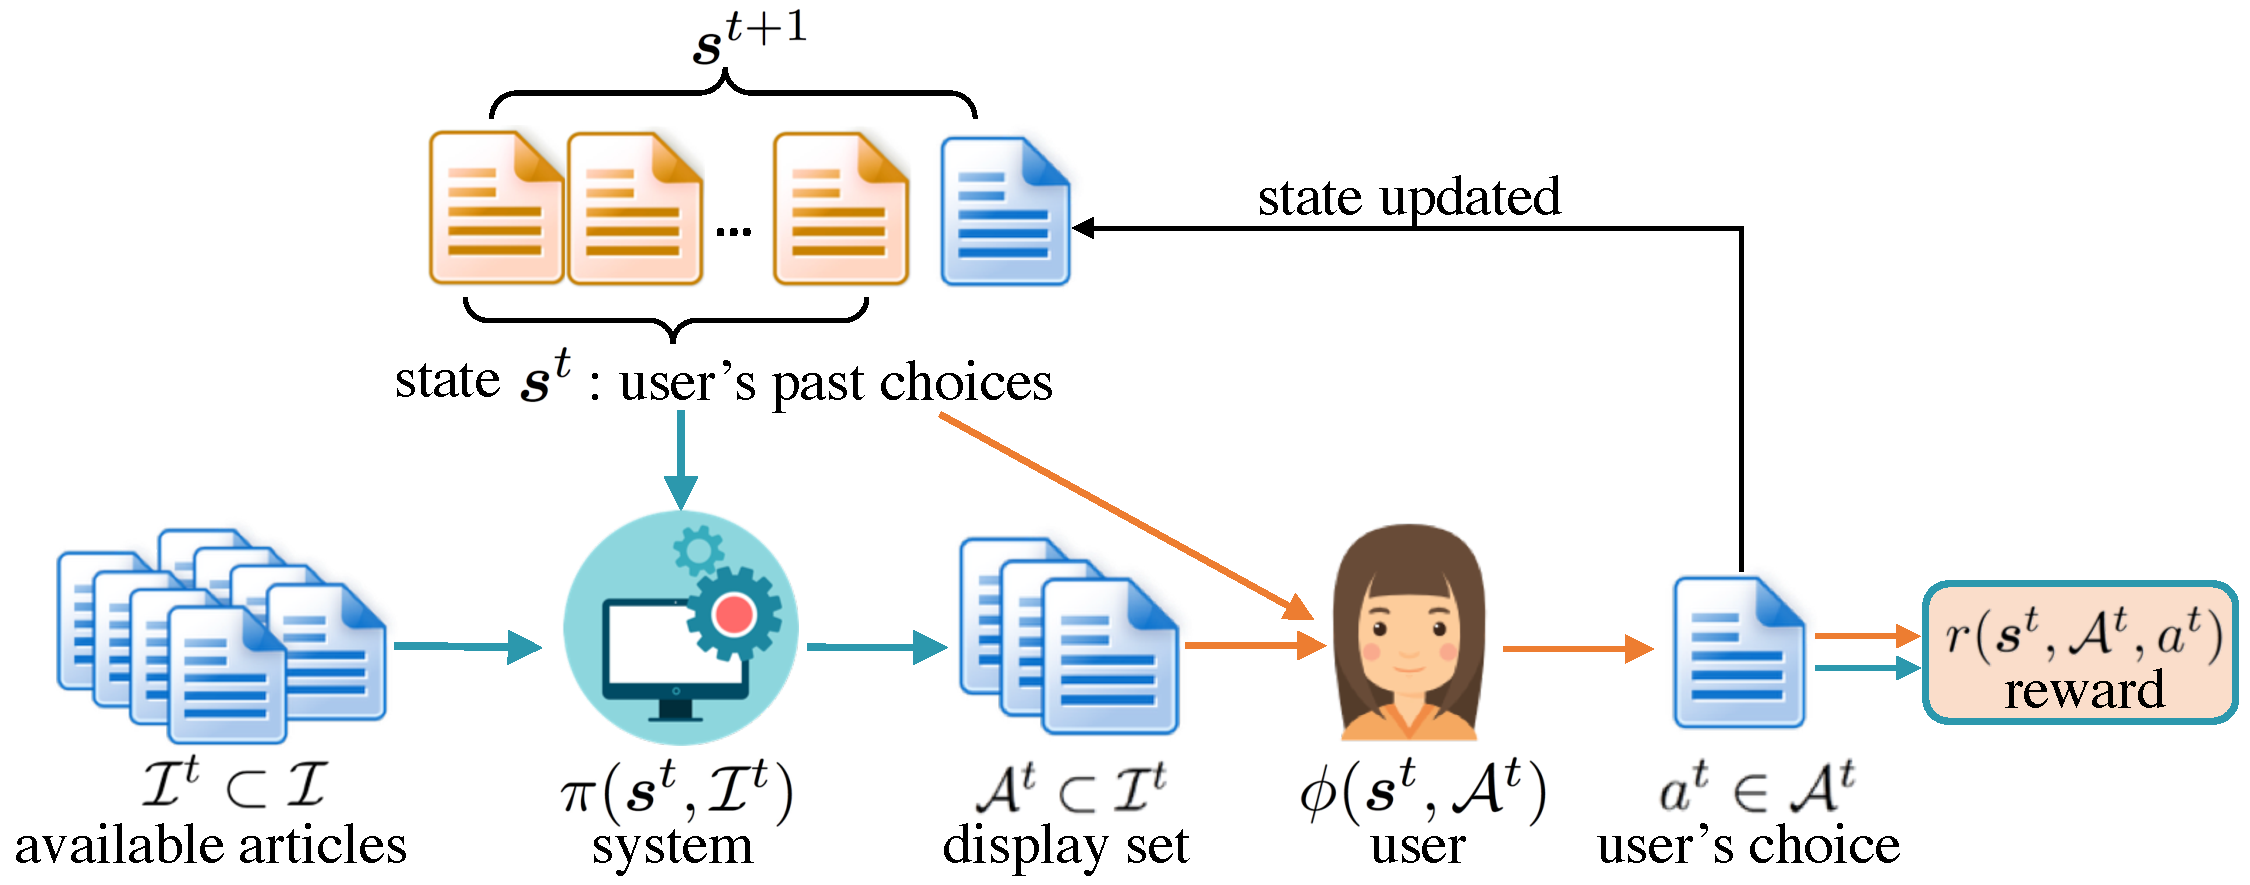
\includegraphics[width=0.75\textwidth]{overallfigure.pdf}
    \vspace{-3mm}
    \caption{An illustration of the interaction between user and recommendation system. Green arrows represent the recommendation framework and orange arrows represent user's framework.
    % \xc{hard to make this figure space efficient... feel free to edit the figure in 'overallfigure.pptx'}
    }
    \label{fig:overall_framework}
    \vspace{-3mm}
\end{figure}{}

\vspace{-3mm}
\section{Generative Adversarial Network for User Behavior}
\vspace{-3mm}

In this section, we will propose a model for the sequence of user clicking behavior\Li{\st{, discussion} and discuss} its parametrization and parameter estimation.  

\vspace{-3mm}
\subsection{User Behavior As Reward Maximization}\label{sec:user_model}
\vspace{-3mm}

We assume that during each pageview, the user is presented with $k$ items, out of which she clicks one. The sequence of items selected by the user before session $t$ is an ordered list of observed features, and we view \Li{\st{it or embedding of it} its embedding} as the state of the user, i.e. $\vs^t := h\left(\mF_\ast^{1:t-1} = [ \vf_\ast^{1},\cdots,\vf_\ast^{t-1} ]\right)$, where $\vf_\ast^\cdot \in \sR^d$ is the feature vector of the selected items, and $h(\cdot)$ is an embedding function. One can also view $\mF^{1:t-1}_\ast$ as a matrix of historical features of clicked items, and similarly one can also define $M$ step historical features of click items as $\mF^{t-M:t-1}_\ast:=[\vf_\ast^{t-M},\cdots,\vf_\ast^{t-1}]$. 

Suppose in pageview $t$, the user is presented with a set of $k$ items $\gA^t = \{a_1, \cdots, a_k \}$ and their associated features $\mF^t = \{\vf^t_1,\cdots, \vf^t_k\}$ by the recommendation system, and a selection $a^t\in \gA^t$ is taken by the user according to her preference function $a^t\sim \phi^*(\vs^t, \gA^t)\in \Delta^{k-1}$ where $\Delta^{k-1}$ is the probability simplex. More specifically, we assume that user clicks items to maximize its own interests. That is we assume that user's clicking probability is the results of the following optimization
{\small \begin{equation}\label{eq:max}
    \textbf{User Model:}~~~~\phi^*(\vs^t,\gA^t) = \arg\max_{\phi \in \Delta^{k-1}} \E_{\phi} \left[r(\vs^t, a^t) \right] -\frac{1}{\eta}\E_{\phi}[R(\phi)],
\end{equation}}
where $R(\phi)$ is a concave regularization function and $\eta$ controls the strength of the regularization. After clicking an item $a^t$, the user state will be updated to $\vs^{t+1} =h\left(\mF_\ast^{1:t}=\{\vf_\ast^{1},\cdots,\vf_\ast^{t-1}, \vf^t_{a^t}\}\right)$. 

{\bf Remark.} We assume the case when the user does not click any item to be a special item and consider its reward as zero or a constant to be learned. Alternatively, it can also be included as an item of zero feature vector, so equation~\eqref{eq:max} can generate this case with simple modification. Besides, when no item is clicked, the state of user will not be updated (i.e., $\vs^{t+1} = \vs^t$). 

% % \Le{combine this paragraph and the paragraph of state update using itemize to better show the overall user behavior model.} 
% \shuang{Need to clarify a few things here:

% 1. Is the $k$ here the same as the $k$ items recommended by agents?

% 2. Then why the degree of the probability simplex is $k$ instead of $k-1$

% 3. Add one more possible choice of action "click none of the recommended items"

% 4. What are the exploitation and exploration referring to for users?}

% \xc{added to remark.}

Furthermore, if we allow $\phi \in \Delta^{k-1}$ to be arbitrary mappings (i.e., not limited in a specific parameter space), the optimization problem in~\eqref{eq:max} has a closed form solution, where user clicks on an item according to an exponential distribution in the follow lemma (See Appendix~\ref{app:proof} for a proof).
\begin{restatable}{lemma}{primelemma}\label{lm:lemma1}
Let the regularization be $R(\phi) = \log(\phi)$ and $\phi \in \Delta^{k-1}$ include arbitrary mappings. Then the optimal solution $\phi^*$ for the problem in~\eqref{eq:max} has a closed form
\begin{equation}\label{eq:exp}
	\phi^\ast(\vs^t,\gA^t)_i = \dfrac{\exp(\eta r(\vs^t, a_i))}{\sum_{a_j \in \gA^t}\exp(\eta r(\vs^t, a_j))}.
\end{equation}
Furthermore, at each time $t$, the user's decision according to her optimal policy $\phi^*$ is equivalent to \Li{\st{he} the} following discrete choice model
{\small \begin{equation}\label{eq:gumbel}
 	a^t = \arg\max_{a \in \gA^t }~\eta\, r(\vs^t, a) + \varepsilon^t,
 \end{equation}}
 where $\varepsilon^t$ follows a Gumbel distribution.
\end{restatable}
This lemma makes it clear that the user essentially greedily picks an item according to its reward function (exploitation), and yet the Gumbel noise $\varepsilon^t$ allows the user to deviate and explore other less rewarding items. Similar model has also appeared in the econometric choice model~\citep{Manski75,McFa73}, but previous econometric models did not take into account diverse features and user state evolution. Furthermore, to the best of our knowledge, such models have not been considered in model-based RL. Furthermore, other regularization $R(\phi)$ can also be used in our framework, which may induce different user behaviors. In these cases, the relations between $\phi^*$ and $r$ are also different, and may not appear in closed form. 
\vspace{-3mm}
\subsection{Model Parameterization}
\vspace{-3mm}
In the following, we will first define the state embedding $\vs^t = h(\mF^{1:t-1}_\ast)$, and then define the reward function $r(\vs^t, a^t)$ based on the state and the embedding of click $a^t$. 

More specifically, we propose to use a simple and effective position weighting scheme for the state embedding. Let $\mW \in \sR^{m\times n}$ be a matrix where the number of rows $m$ correspond to the number of history steps to take into account, and each of the $n$ columns will correspond to one set of importance weights on positions. Then the embedding map $h$ can be designed as 
{\small \begin{equation}
    \label{eq:state_embedding}
    \vs^t = h(\mF^{1:t-1}_\ast) := vec \left[\, \sigma \left(\, \mF_*^{t-m:t-1} \mW + \mB \,\right)\, \right]~~\in~~\sR^{dn\times 1}, 
\end{equation}}
where $\mB\in \sR^{d\times n}$ is a bias matrix, $\sigma(\cdot)$ is a nonlinear activation function such as the ReLU and ELU unit applied elementwisely to its arguments, and $vec[\cdot]$ turns the input matrix into a long vector by concatenating the matrix columns.
Alternatively, one can also use an LSTM to capture the history. However, the advantage of our position weighting parametrization is that the history embedding is obtained by a shallow network which is more efficient for forward computation and gradient backpropagation than recurrent networks. 

The user clicks $a^t$ corresponds to an item with feature $\vf_{a^t}^t$. Thus we will use $\vf_{a^t}^t$ as the surrogate for user click and parametrize the reward function and user behavior model as 
{\small \begin{equation}
    r(\vs^t, a^t) := \vr^\top \sigma \left(\, \mV \left[
    \begin{matrix}
        \vs^t \cr
        \vf_{a^t}^t
    \end{matrix}
    \right] + \vb \, \right),~~~
    \phi(\vs,\gA^t) \propto \exp\left( 
    {\vr'}^{\top} \sigma \left(\, \mV' \left[
    \begin{matrix}
        \vs^t \cr
        \vf_{a^t}^t
    \end{matrix}
    \right] + \vb' \, \right)    
    \right)     
\end{equation}}
where $\mV,\mV' \in \sR^{\ell \times (dn+d)}$ are weight matrices, $\vb,\vb' \in \sR^{ 1 \times (dn+d)}$ are bias vectors and $\vr,\vr' \in \sR^{\ell}$ are the final regression parameter. See Figure \ref{fg:usermodel} for an illustration of the overall parametrization. \Li{It seems that $\vr'$ here is used as the parameters of neural network, which is easy to cause misunderstanding with the reward function $r$ despite they are two different notations.}
\begin{figure}[htbp]
    \vspace{-3mm}
  \begin{minipage}[c]{0.53\textwidth}
    \centering
    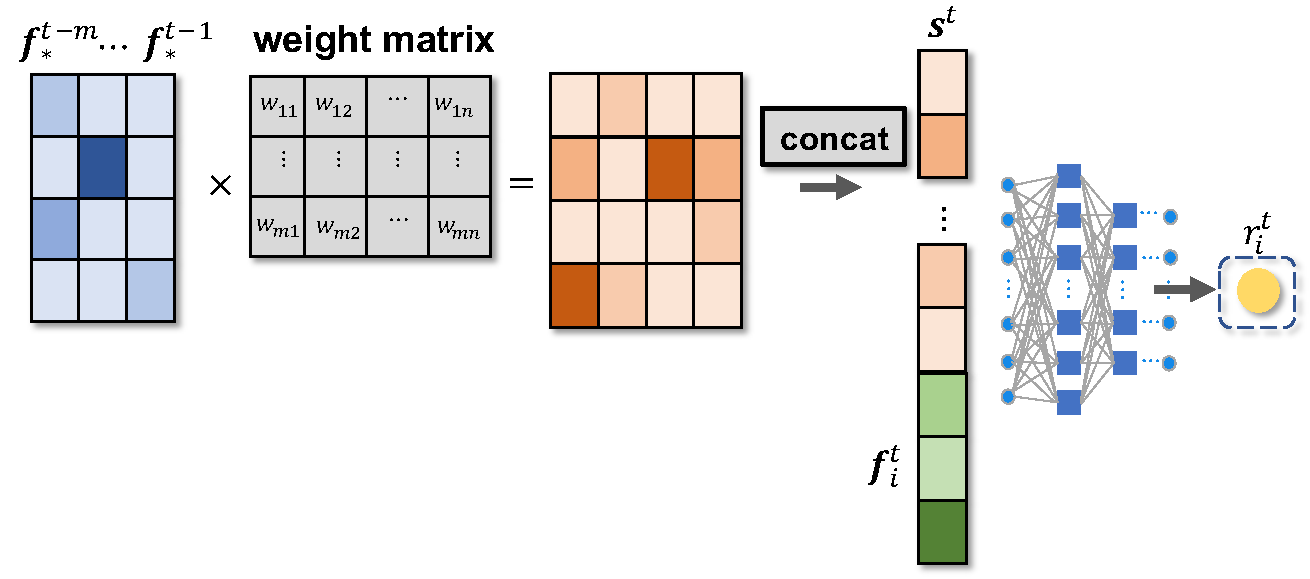
\includegraphics[width=\textwidth]{Figs/PABOW.pdf}
  \end{minipage}
  \begin{minipage}[c]{0.42\textwidth}
    \centering
    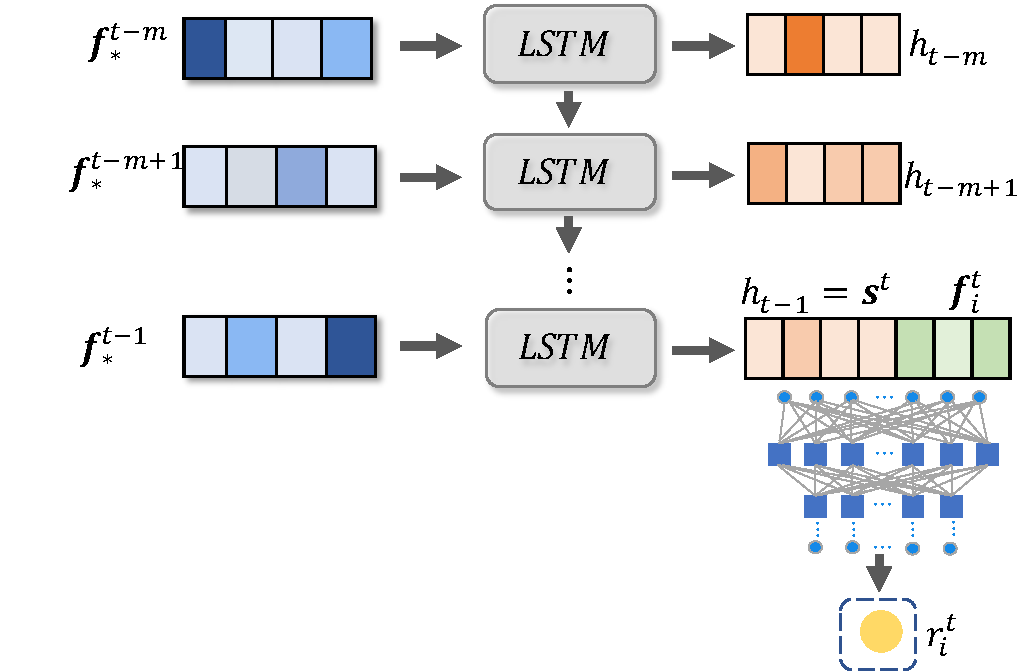
\includegraphics[width=\textwidth]{Figs/LSTM.pdf}
  \end{minipage}\hfill
    \vspace{-3mm}
  \caption{\small Architecture of our GAN model with reward function and user behavior model parameterized similarly by either position weight (PW) or LSTM. 
    }
    \label{fg:usermodel}
    \vspace{-3mm}
\end{figure}

\vspace{-3mm}
\subsection{Learning User Behavior Model}
\vspace{-3mm}

In practice, both the user reward function $r(\vs^t,a^t)$ and the behavior model $\phi(\vs^t, \gA^t)$ are unknown and need to be estimated from data. Given a sequence of $T$ observed user clicks, $\{a^1_{true},a^2_{true},\ldots,a^T_{true}\}$ and the corresponding item features $\{\vf_\ast^1, \vf_\ast^2, \ldots, \vf_\ast^T\}$, we can estimate the user utility and behavior model by solving the following mini-max optimization 
% \xc{equation slightly changed. i think this is more general.}
{\small \begin{equation}\label{eq:std-minmax}
	\min_{\theta \in \Theta} \left(\max_{\phi\in \Phi}  \E_{\phi} \left[\sum_{t=1}^Tr_{\theta}(\vs^t_{true}, a^t) -\frac{1}{\eta}R(\phi)\right]\right)-\sum_{t=1}^T r_{\theta}(\vs^t_{true}, a^t_{true})
\end{equation}}
where $\theta$ denotes all parameters in the $r$ function, $\Phi \subset \{\phi:\gS \times {\gI \choose k} \mapsto \Delta^{k-1}\}$ denotes a family of mappings, and we use $\vs^t_{true}=\{\vf_\ast^1,\ldots,\vf_\ast^{t-1}\}$ to emphasize that this is observed in the data. 
The meaning of the optimization problem is that 
a good reward function should give the observed user behavior higher reward than the user behavior model, and thus the user model can approach the real user behavior by maximizing this reward function. 

The mini-max optimization problem in~\eqref{eq:std-minmax} can be  solved by iteratively updating the $\phi$ and $r_{\theta}$, but the process may be unstable due to the non-convex problems.  
% \st{If we allow $\sigma^t \in \Delta^{k-1}$ to include all possible mappings, the optimization problem in}~\eqref{eq:std-minmax}\st{ is equivalent to maximum likehihood estimation as in the following lemma.}  
\xinshi{We will explain how we can make use of a special closed form to help initialize the mini-max optimization after the statement of the following lemma.} See Appendix~\ref{app:proof} for a proof.   
% To learn the user policy, we tend to modify~\eqref{eq:std-minmax} to~\eqref{eq:modify-minmax}.

% \xc{explain why~\eqref{eq:modify-minmax}: (1) In reality, user is unable to optimize her cumulative reward without observing those items displayed to her in the future. (2) As a recommender, we do not benefit much from generating a whole trajectory of user's choices given user's initial states, because we can always observe her current states before we make recommendation.}

% \begin{equation}\label{eq:modify-minmax}
% \min_{\theta \in \Theta} \Big(\max_{\pi\in \Pi} \E_{\pi} \sum_{t=1}^T r_{\theta}(\vs^t_{true}, a^t) -\frac{1}{\eta}\E_{\pi}R(\pi)\Big)-\sum_{t=1}^T r_{\theta}(\vs^t_{true}, a^t_{true})
% \end{equation}
\begin{restatable}{lemma}{secondlemma}\label{lm2:mle}
Consider the case when regularization is defined as $R(\phi) = \log(\phi)$ and $\Phi$ includes all mappings from $\gS \times {\gI \choose k}$ to $\Delta^{k-1}$. Then the optimization problem in~\eqref{eq:std-minmax} is equivalent to the following maximum likelihood estimation
{\small \begin{equation}\label{eq:mle}
	\max_{\theta \in \Theta}~\prod_{t=1}^T \dfrac{\exp(\eta r_{\theta}(\vs_{true}^t, a^t_{true}))}{\sum_{a^t \in \gA^t}\exp(\eta r_{\theta}(\vs_{true}^t, a^t))}.
\end{equation}}
 \end{restatable}
%  \xc{I fail to come up with a good argument here....don't know how to emphasize the gan...instead of mle..}
This lemma enables us to learn a $\theta^*$ in a more stable and efficient way by solving a single maximization problem. We can simply apply standard algorithms such as SGD or ADAM to find an approximate solution $\hat{\theta}^*$. Then we can use this $\hat{\theta}^*$ as the initialization for the optimization problem~\eqref{eq:std-minmax} with other $R(\phi)$.   
% Furthermore, if we use other regularization function $R(\phi)$, the original optimization problem in~\eqref{eq:std-minmax} can not be expressed as~\eqref{eq:mle}, and we need to optimize both $\theta$ and $\phi^t$. In this case, we can use $\hat{\theta}^*$ estimated from maximum likelihood to initialize the $\theta$ in this new optimization problem. 

% an approximately optimal solution $\hat{\theta}$ to~\eqref{eq:mle} by SGD. With many experimental trails, we find the learned $\hat{\theta}^*$ a good initialization of $\theta$ for the mini-max optimization problem and help to stablize the mini-max training process.
% \Le{Say something about why this is interesting .. More stable training etc ...} 
% \Le{How does $a_{true}$ get into the expression?} 
% \xc{the $\min_{\theta}$ in minmax is equivalent to min negative log likelihood. add a brief proof in appendix later}
\vspace{-3mm}
\section{Cascading Q-networks for Recommendation Policy}
\vspace{-3mm}

Using the estimated user behavior model and the corresponding reward function as the simulation environment, we can then use reinforcement learning to obtain a recommendation policy. Note that the recommendation policy needs to deal with a {\it combinatorial action space} $\gI \choose k$, where each action is a set of $k$ items chosen from a \Li{\st{larger} large} set $\gI$ of $K$ candidates. \Li{$K$ is not defined.}
Two challenges associated with this problem include the potentially high computational complexity of the combinatorial action space and the development of a framework for estimating the long-term reward (the Q function) from a combination of items. Our contribution is designing a novel cascade of Q-networks consistent with each other for handling the combinatorial action space. Based on this cascade of Q-networks, we can also design an algorithm to estimate them from interaction with the environment. 

% \shuang{
% Short: Using the developed user behavior model as the simulation environment, we design a factorized deep Q-network (DQN) algorithm to obtain a recommendation policy. 

% Note: the following paragraphs are from Lihong Li's KDD paper:

% More specifically, we consider tasks with a combinatorial action space, where each action is a set of multiple interdependent sub-actions. Only a limited number of number of items can be recommended. Different from typical reinforcement learning, the action space is combinatorial since an action corresponds to a set of items (sub-actions) chosen from a larger set of candidates. Two challenges associated with this problem include the potentially high computational complexity of the combinatorial action space and the development of a framework for estimating the long-term reward (the Q function) from a combination of sub-actions. Here we focus on the second problem, exploring different deep neural network architectures in an effort to efficiently account for the potential redundancy and/or temporal dependency of different sub-actions in relation to the state space. We sidestep the computational complexity issues by...The contribution is the development of a novel deep reinforcement learning architecture for handling a combinatorial action space. }

% In this section, we will learn a policy for the recommendation system based on the user behavior model. The goal of the recommendation policy is to maximize the expected long term reward of the user. To realize this goal in the reinforcement learning framework, we assume that the reward to the recommendation system is the same as that of the user, and the environment dynamics will correspond to the user behavior model learned in the previous section; The user's behavior will be influenced by the actions of the recommendation system and potentially being led to achieve better long term rewards. That is we want to learn an optimal recommendation policy $\pi(\vs)$ which takes the user's state $\vs$ and chooses $k$ items to display. 

% Since each time the recommendation system needs to choose a set of $k$ items from a potentially large pool of items, we will design a factorized action-value function $Q$ to address this challenge. Furthermore, we will will adapt the Q-learning method to estimate this factorized $Q$ function. 

\vspace{-3mm}
\subsection{Cascading Q-Networks}
\vspace{-3mm}

We assume that each time when a user visits the online platform, 
%In each session (or interaction with the user),\Le{Session may not be a good word, since Session could mean mutiple displays} 
the recommendation system need to choose a subset $\gA$ of $k$ items, i.e., $\gA \subset \gI$. We will use the Q-learning framework where an optimal action-value function $Q^*(\vs,\gA)$ will be learned and satisfies
% \begin{equation}\label{eqn:bellman}
% 	Q^*(\vs^t, \gA^t) =\E_{a^t\sim \sigma(\vs^t)}\left[r(\vs^t, a^t)\right] + \gamma  \E_{a^t\sim\sigma(\vs^t),\vs^{t+1}\sim P(\vs^{t+1}|\vs^t,a^t)}\left[\gAx_{\mA'}Q^*(\vs^{t+1}, ')\right].
% \end{equation}
{\small \begin{equation}\label{eqn:bellman}
	%Q^*(\vs^t, \gA^t) = \underbrace{\E_{\sigma}\left[r(\vs^t, a^t)\right]}_{:=Rwd(\vs^t, \gA^t)} + \gamma  \E_{\sigma}\left[\max_{\gA'\subset \gI}Q^*(\vs^{t+1}, \gA')\right],~~a^t \in \gA^t.
		Q^*(\vs^t, \gA^t) =\E\left[r(\vs^t, \gA^t, a^t) + \gamma  \max_{\gA'\subset \gI}Q^*(\vs^{t+1}, \gA')\right],~~a^t \in \gA^t.
\end{equation}}
% The action $\gA^t$ corresponds to $k$ items chosen from $K$ items.  \Le{It is equivalent to the notation $\mF^t=\{\vf^t_1,\cdots, \vf^t_k\}$. Add this earlier}. 
% Note that the value $r(\vs^t, a^t)$ depends on the feature content of the recommendation action $\gA^t$, so to simplify notation, we write $Rwd(\vs^t, \gA^t):=\E_{\sigma}\left[r(\vs^t, a^t)\right]$.
Once the action-value function is learned, an optimal policy for recommendation can be obtained as
{\small \begin{equation}\label{eq:policy}
	\pi^\ast(\vs^t, \gI^t)=\arg\max_{\gA^t\subset \gI^t}Q^*(\vs^t, \gA^t), 
\end{equation}}
where $\gI^t \subset \gI$ is the set of items available at time $t$. Furthermore, we assume that once an item is clicked by an user, it becomes unavailable and will be excluded from being recommended again. 
The challenge is that the action space of the recommendation system contains ${K \choose k}$ many choices, which can be very large even for moderate $K$ (e.g. 1000) and $k$ (e.g. 5). Furthermore, an item put in different combinations can have different probability of being clicked, which is indicated by the user model and is in line with reality. For instance, interesting items may compete with each other for user attention. Thus, the policy in~\eqref{eq:policy} will be very expensive to compute. To address this challenge, we will design not just one but a set of $k$ related Q-functions which will be used in a cascading fashion for finding the maximum in~\eqref{eq:policy}. 

Let an recommendation be $\gA=\{a_1, a_2,\cdots, a_k\}$ and the optimal action given state $\vs$ be $\gA^* =\{a_1^*, a_2^*, \cdots, a_k^*\} =\arg\max_{\gA} Q^*(
\vs, \gA)$. The key idea of our cascading Q-function framework comes from the following fact:
{\small \begin{equation}\label{eq:max_decomp}
\max_{a_1,a_2,\cdots,a_k}Q^*(\vs,a_1,a_2,\cdots,a_k) = \max_{a_1}\left( \max_{a_2,\ldots,a_k}Q^*(\vs,a_1,a_2,\cdots,a_k) \right),
\end{equation}}
which also implies that there is a cascade of mutually consistent $Q^{1*},Q^{2*},\ldots,Q^{k*}$ such that: 
{\small \begin{align*}
    a_1^* =\arg \max_{a_1}Q^{1*}(\vs, a_1) & \quad\text{with}\quad\displaystyle Q^{1*}(\vs, a_1):=\max_{a_2,\cdots,a_k}Q^*(\vs,a_1,\cdots, a_k),  \\
      a_2^* =\arg \max_{a_2}Q^{2*}(\vs, a_1^*, a_2) & \quad\text{with}\quad \displaystyle Q^{2*}(\vs, a_1, a_2):=\max_{a_3,\cdots,a_k}Q^*(\vs,a_1,\cdots, a_k), \\
      \cdots & \cdots \nonumber\\
      a_k^* = \arg \max_{a_k}Q^{k*}(\vs, a_1^*,\cdots,a_{k-1}^*, a_k) & \quad\text{with}\quad Q^{k*}(\vs, a_1, \cdots,a_k):=Q^*(\vs,a_1,\cdots, a_k).  
\end{align*}}
Thus, if we have access to all these $Q^{j*}$ functions, then we can obtain an optimal action in $O(k|\gI|)$ computations by applying these function in a cascading manner. See algorithm~\ref{alg:argmax_q} and Figure~\ref{fig:qnetwork} for a summary. However, these cascade of $Q^{j*}$ functions are usually not available and need to be estimated from data. 
% \Le{Shuang: nice minipage. can you make the figure 3 shorter and the fontsize for Q larger and darker? 4-boxes to 3 boxes!}

\vspace{-3mm}
\subsection{Parametrization and Estimation of Cascading Q-Networks} 
\vspace{-3mm}

Note that the set of $Q^{j*}$ functions need to satisfy a large set of constraints which may not be easy to strictly enforce. That is at the optimal point, the value of $Q^{j*}$ is the same as $Q^*$ for all $j$, i.e., 
{\small \begin{equation}
    \label{eq:constraints}
        Q^{j*}(\vs, a_1^*, \cdots, a_j^*) = Q^*(\vs,a_1^*,\cdots,a_k^*),\quad \forall j=1,\ldots, k.
\end{equation}}
Instead of coding these constraints in our neural network parametrization, we will take them into account in a soft and approximate way in our model fitting process. 

More specially, we will use the same embedding for the state $\vs$ as in~\eqref{eq:state_embedding}, and parametrize each $Q^{j*}$ function as
{\small \begin{equation}
    \widehat{Q^{j}}(\vs, a_{1:j-1}^*, a_j; \Theta_j) = \vq_j^\top \sigma \left( \mL_j\,
        \left[
            \vs^\top,\,  
            \vf_{a_1^*}^\top,\, 
            \ldots,\,
            \vf_{a_{j-1}^*}^\top,\,
            \vf_{a_j}^\top
        \right]^\top
        +\, \vc_j
    \right),~~\forall j=1,\ldots,k
\end{equation}}
where $\mL_j \in \sR^{\ell\times(dn+dj)}$, $\vc_j \in \sR^{\ell}$, and $\vq_j \in \sR^{\ell}$ are the set $\Theta_j$ of parameters. Now the problem left is how we can estimate these functions $\widehat{Q^{j}}$ and take into account constraints in~\eqref{eq:constraints}. 

Different from standard Q-learning, our cascading Q-learning process will then be learning $k$ parametrized functions $\widehat{Q^j}(\vs^t, a_{1:j-1}^*, a_j; \Theta_j)$ as approximations of $Q^{j*}$. To enforce the constraints in~\eqref{eq:constraints} in a soft and approximate way, we can define the loss as
{\small \begin{equation}
\label{eq:loss}
\big(y- \widehat{Q^j} \big)^2,~\text{where}~y= r(\vs^t, \gA^t, a^t) + \gamma \widehat{Q^{k}}(\vs^{t+1}, a_1^*,\cdots,a_k^*; \Theta_k),~ \forall j=1,\ldots,k.
\end{equation}}
That is all $\widehat{Q^j}$ is fitting against the same target. Then the parameters $\Theta_k$ can be updated by performing gradient \Li{descent} steps over the above loss. 
% $\big(y- \widehat{Q^j} \big)^2$, where we apply the same value $y= r(\vs^t, \gA^t, a^t) + \gamma \widehat{Q^{k}}(\vs^{t+1}, a_1^*,\cdots,a_k^*; \Theta_k)$ for each $j$ and update the parameters $\Theta_j$ by performing gradient steps. 

The overall cascading Q-learning algorithm is summarized in Algorithm~\ref{alg:dqn} in Appendix~\ref{app:algo}, where we employ the cascading $Q$ functions to search the optimal action efficiently (line~\ref{line:argmax}). Besides, both the experience replay~\citep{MniKavSilGraetal13} and $\epsilon$-exploration techniques are applied. The system's experiences at each time-step are stored in a replay memory set $\gM$ (line~\ref{line:exp_replay1}) and then a minibatch of data will be sampled from the replay memory to update $\widehat{Q^j}$ (line~\ref{line:exp_replay2} and~\ref{line:exp_replay3}). An exploration to the action space is executed with probability $\epsilon$ (line~\ref{line:epsilon-greedy}).

\begin{tabular}{cc}
\begin{minipage}{.5\textwidth}
\begin{algorithm}[H]
\caption{Search using $\widehat{Q^{j}}$ Cascades}
\label{alg:argmax_q}
\begin{algorithmic}[1]
\Function{argmax\_Q}{$\vs, \gA, \Theta_1,\cdots,\Theta_k$}
    \State Let $\gA^*$ be empty.
    \State $\gI = \gA \setminus{\vs}$ \Comment{remove clicked items.}
    \For{$j=1$ to $k$}
    	\State $\displaystyle {a}_j^*=\argmax_{a_j\in \gI \setminus {\gA^*} }\widehat{Q^{j}}(\vs, {a}_{1:j-1}^*, a_j; \Theta_j)$
    	\State Update ${\gA}^* = {\gA}^* \cup \{{a}_j^* \}$
    \EndFor
    \State \Return ${\gA}^* = ({a}_1^*,\cdots,{a}_k^*)$
\EndFunction
\end{algorithmic}
\end{algorithm}
\end{minipage} &
\begin{minipage}{.5\textwidth}
\centering
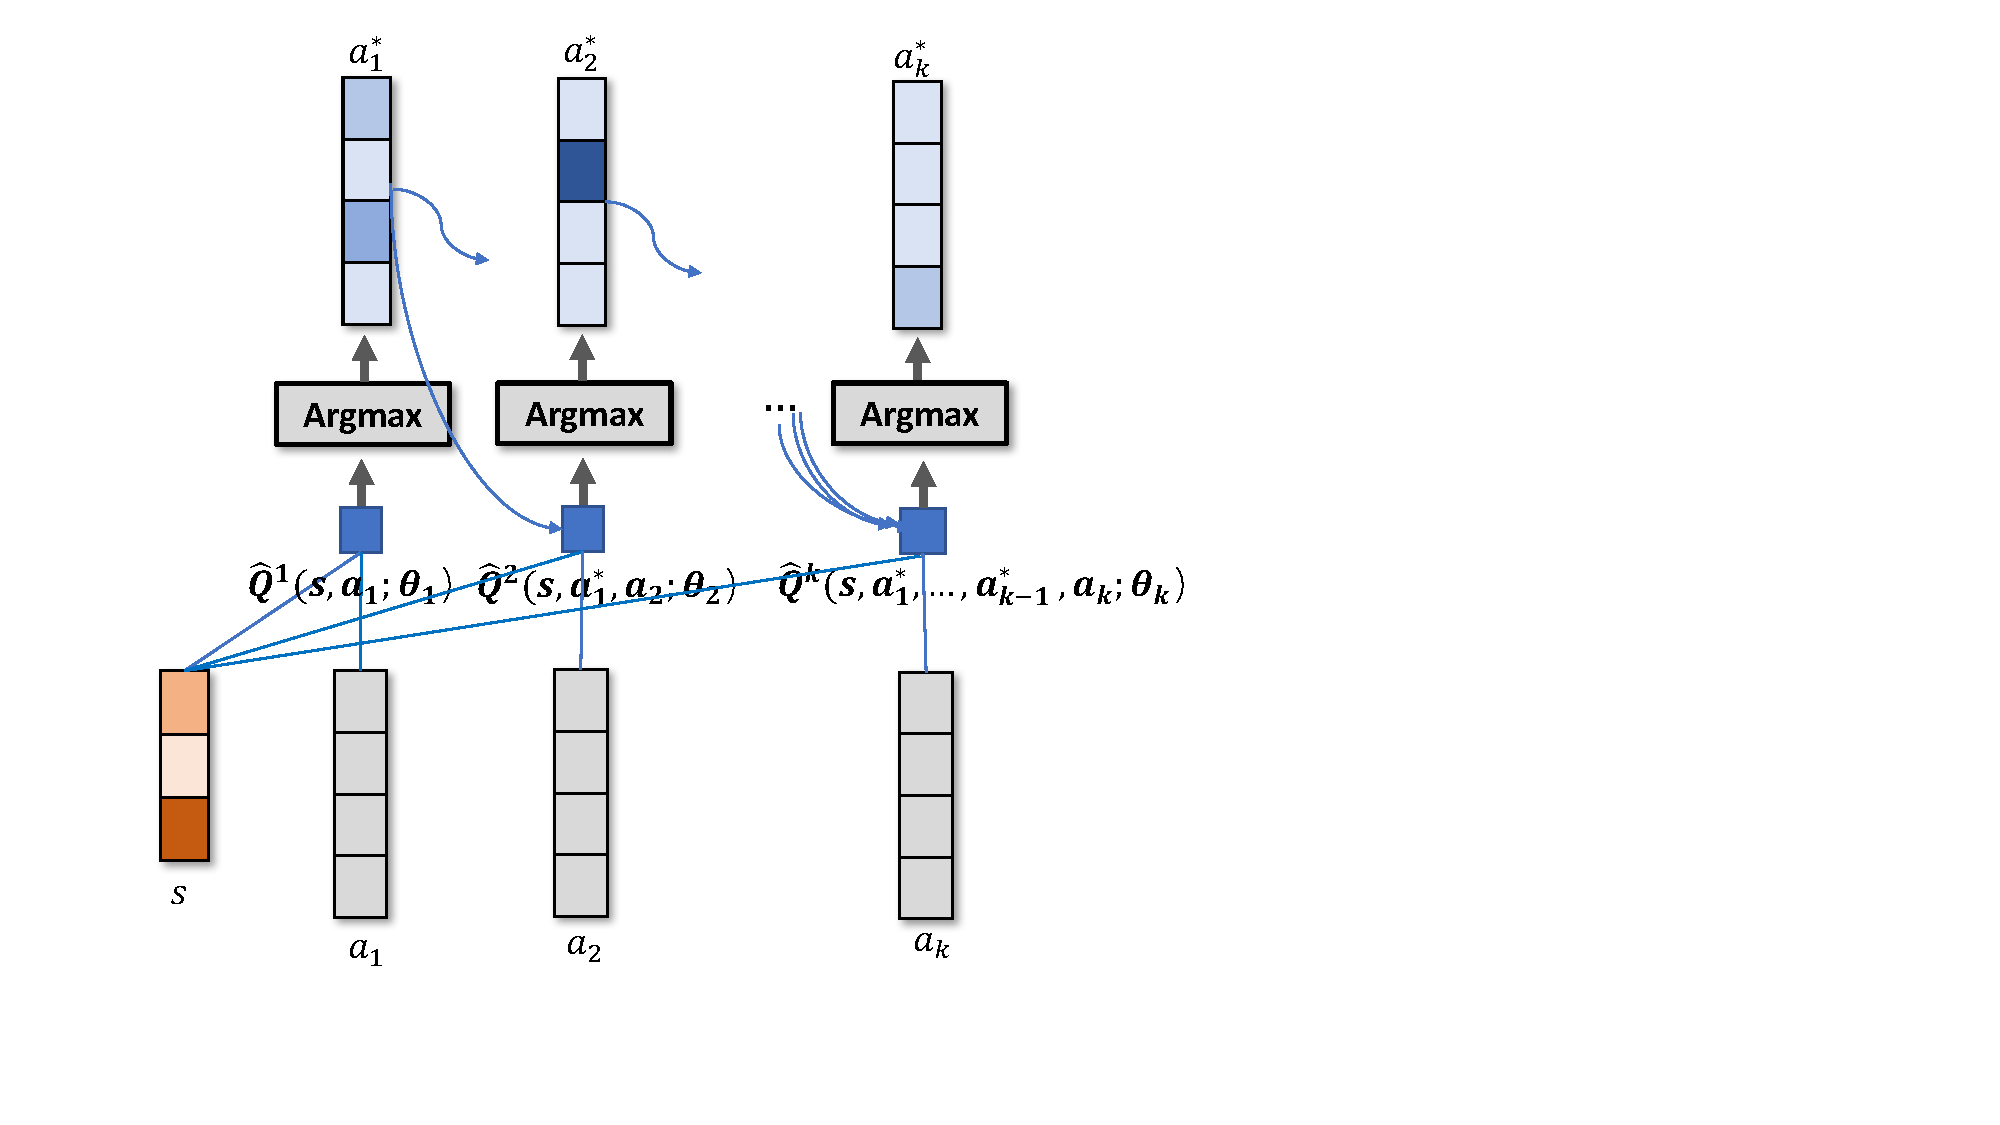
\includegraphics[width=0.8\textwidth]{Figs/Qnetwork_new.pdf}
\vspace{-3mm}
\captionof{figure}{Cascading Q-networks}
\label{fig:qnetwork}
\vspace{-3mm}
\end{minipage}
\end{tabular}

\vspace{-3mm}
\section{Experiments}
\vspace{-3mm}

We conduct three sets of experiments to evaluate our user model (called {\textbf GAN} model) and the resulting RL recommendation policy. {\bf (1)} The first set of experiments in section~\ref{sec:experiment1} show that GAN is a better predictive user model. By taking both the context where the item is displayed in and the evolution of user's interest into account, GAN outperforms other baseline models in terms of both likelihood and precision. {\bf (2)} In section~\ref{sec:experiment2} we compare the recommendation policies developed from different user models. It is revealed from experiments that recommendation policies generated from GAN model can not only help users achieve higher long term reward but also help the system achieve higher click rate. {\bf (3)} In section~\ref{sec:experiment3} we test how recommendation policies can benefit from GAN model to better capture users' interest with fewer interactions. A comparison is made among RL policy with two versions of our GAN model (GAN(PW) and GAN(LSTM)), RL policy without GAN model and multi-arm bandit algorithm which does not make an assumption on user behavior.

\vspace{-3mm}
\subsection{Dataset and feature description}
\vspace{-3mm}

We will use two real world datasets for our experiments: {\bf (1) MovieLens public dataset} and {\bf (2) an online news article recommendation dataset from Ant Financial}. The datasets are either preprocessed or collected to follow our recommendation setting in Figure~\ref{fig:overall_framework}. More details can be found in Appendix~\ref{app:dataset}. 

\vspace{-3mm}
\subsection{Predictive performance of user model}\label{sec:experiment1}
\vspace{-3mm} 

A series of models are designed to predict user behavior by utilizing the interaction data with users, among which logistic regression (LR) and collaborative filtering (CF) type models are popular. Besides, collaborative competitive filtering (CCF) model significantly outperforms standard CF approaches as reported by~\cite{YanLonSmoEtal11b}. Thus, we choose the most widely used LR model and the advanced CF model (CCF) as our baseline: {\bf (1) Logistic regression (LR)}. The click-through rate(CTR) likelihood function can be defined using logistic function as $p_i = \frac{1}{1+\exp{(-r(\vf_i))}}$, where $r(\cdot)$ is a utility/reward function learned by optimizing $\sum_{i\in \gC}\log \big(1+\exp(-r(\vf_i))\big) + \sum_{i \not\in \gC}\log\big(1+\exp(r(\vf_i))\big)$ where $\gC$ is the set of clicked items;
{\bf (2) Collaborative competitive filtering (CCF)}. CCF predicts users' action by comparing the items in the current display set $\mF$. More precisely, the likelihood formulation of CCF is $p_i = \exp(r(\vf_i))/\sum_{\vf_j \in \mF }\exp(r(\vf_j))$.

GAN, CCF, and LR formulate the probability distribution of user behavior in different ways. For both datasets, we randomly split the users into train(50\%), validation(12.5\%) and test(37.5\%) subsets. The predictive performances are only accessed on users in test set and all results shown in this section are averaged over 5 random splits. We consider the following metrics to evaluate the predictive performance of each user model and report results in table~\ref{tb:user_model}.

\begin{itemize}[noitemsep,nolistsep,leftmargin=*]
\item {\bf NLL} is the negative log-likelihood loss value averaged over all users in the test set, $\frac{1}{N}\sum_{u=1}^{N}\frac{1}{T_u}\sum_{t=1}^{T_u} -\log p_{u,i^*}^t$, where $i^*$ is the item clicked by the user observed in the data, $T_u$ is number of events associated with user $u$ and $p_{u,i^*}^t$ is the probability that $u$ clicks item $i^*$ at time $t$. Different user models formulate the probability $p_{u,i^*}^t$ in different ways.

\item {\bf Prec@k} is top-$k$ precision. When a user clicks on one of the displayed items, we count it as an event. For each event, the user model can rank the displayed items by likelihood. Prec@k is the proportion of top-$k$ likelihood items that are truly clicked by the user. An average is taken over all events for each user first before average over all users.

\end{itemize}
\begin{table}[ht!]
\vspace{-1mm}
\caption{\small Predictive performance evaluation: loss and precision of LR, CCF and GAN models assessed on a test set of 25,000 users for the news article dataset and 500 users for MovieLens dataset.}
\label{tb:user_model}
\vspace{-3mm}
\begin{center}
\resizebox{\textwidth}{!}{\begin{tabular}{c|ccc|ccc}
\hline
& \multicolumn{3}{c}{(1) Ant Financial news dataset} & \multicolumn{3}{|c}{(2) MovieLens dataset}\\
\hline 
Model  &\multicolumn{1}{c}{NLL} & prec@1 & prec@2 & \multicolumn{1}{c}{NLL} & prec@1 & prec@2 
\\
\hline
LR    &2.017($\pm$0.007) & 0.375($\pm$0.002) & 0.609($\pm$0.001) &0.743($\pm$0.001) &0.615($\pm$0.007) &0.738($\pm$0.012) \\
CCF    &1.457($\pm$0.003) & 0.377($\pm$0.001) & 0.611($\pm$0.001) &1.164($\pm$0.009)&0.657($\pm$0.008)& 0.752($\pm$0.011)\\
GAN({\footnotesize PW}) & {\bf 1.368}($\pm$0.001) & {\bf 0.419}($\pm$0.001) & {\bf 0.658}($\pm$0.001) & {\bf 1.141}($\pm$0.013) & {\bf 0.666}($\pm$0.007) & {\bf 0.754}($\pm$0.013)\\
GAN(lstm) & {\bf 1.365}($\pm$0.001) & {\bf 0.421}($\pm$0.002) & {\bf 0.659}($\pm$0.002) & {\bf 1.124}($\pm$0.021) & {\bf 0.674}($\pm$0.005) & {\bf 0.763}($\pm$0.012)\\
\hline
\end{tabular}}
\end{center}
\vspace{-3mm}
\end{table}
As shown in table~\ref{tb:user_model}, our GAN user model significantly performs better than baseline models for click predictions. It is noted that the loss of LR is much lower than other models in the MovieLens dataset. This could be caused by the feature reduction process, since we learn the wide\&deep layers by minizing the loss function of LR. The learned reduced features tend to achieve a lower loss for LR model. Besides, by comparing the results of GAN(PW) and GAN(lstm), we find that the position weighted(PW) scheme performs almost the same as the LSTM version, but PW is more favorable due to its simple architecture and efficiency. \emph{Thus in the rest of the paper, we will use GAN(PW) for experiments and simply referring it as GAN.} 

Another interesting comparison is shown in Figure~\ref{fg:traj} and more similar figures are provided in Appendix~\ref{app:exp_usermodel}. The blue curve is the trajectory of a user's actual choices of movies over time. The orange curves are simulated trajectories predicted by GAN and CCF. More specifically, at each time $t$ we collect the item with highest likelihood estimated by each model to form a predicted trajectory. To capture the evolution of user's interest, we perform k-means clustering on movie feature vectors to separate the movies into 80 categories. Each data point $(t, c)$ on the curve represents time step $t$ and the category $c$ of the item clicked by the user.  The upper sub-figure reveals that GAN performs much better as time goes by. By contrast, the items predicted by CCF as shown in the lower sub-figure are concentrated consistently on several categories. This indicates an obvious drawback of static model - it fails to capture the evolution of user's interests. 

\begin{figure}[htbp]
\vspace{-3mm}
  \begin{minipage}[c]{0.6\textwidth}
    \centering
    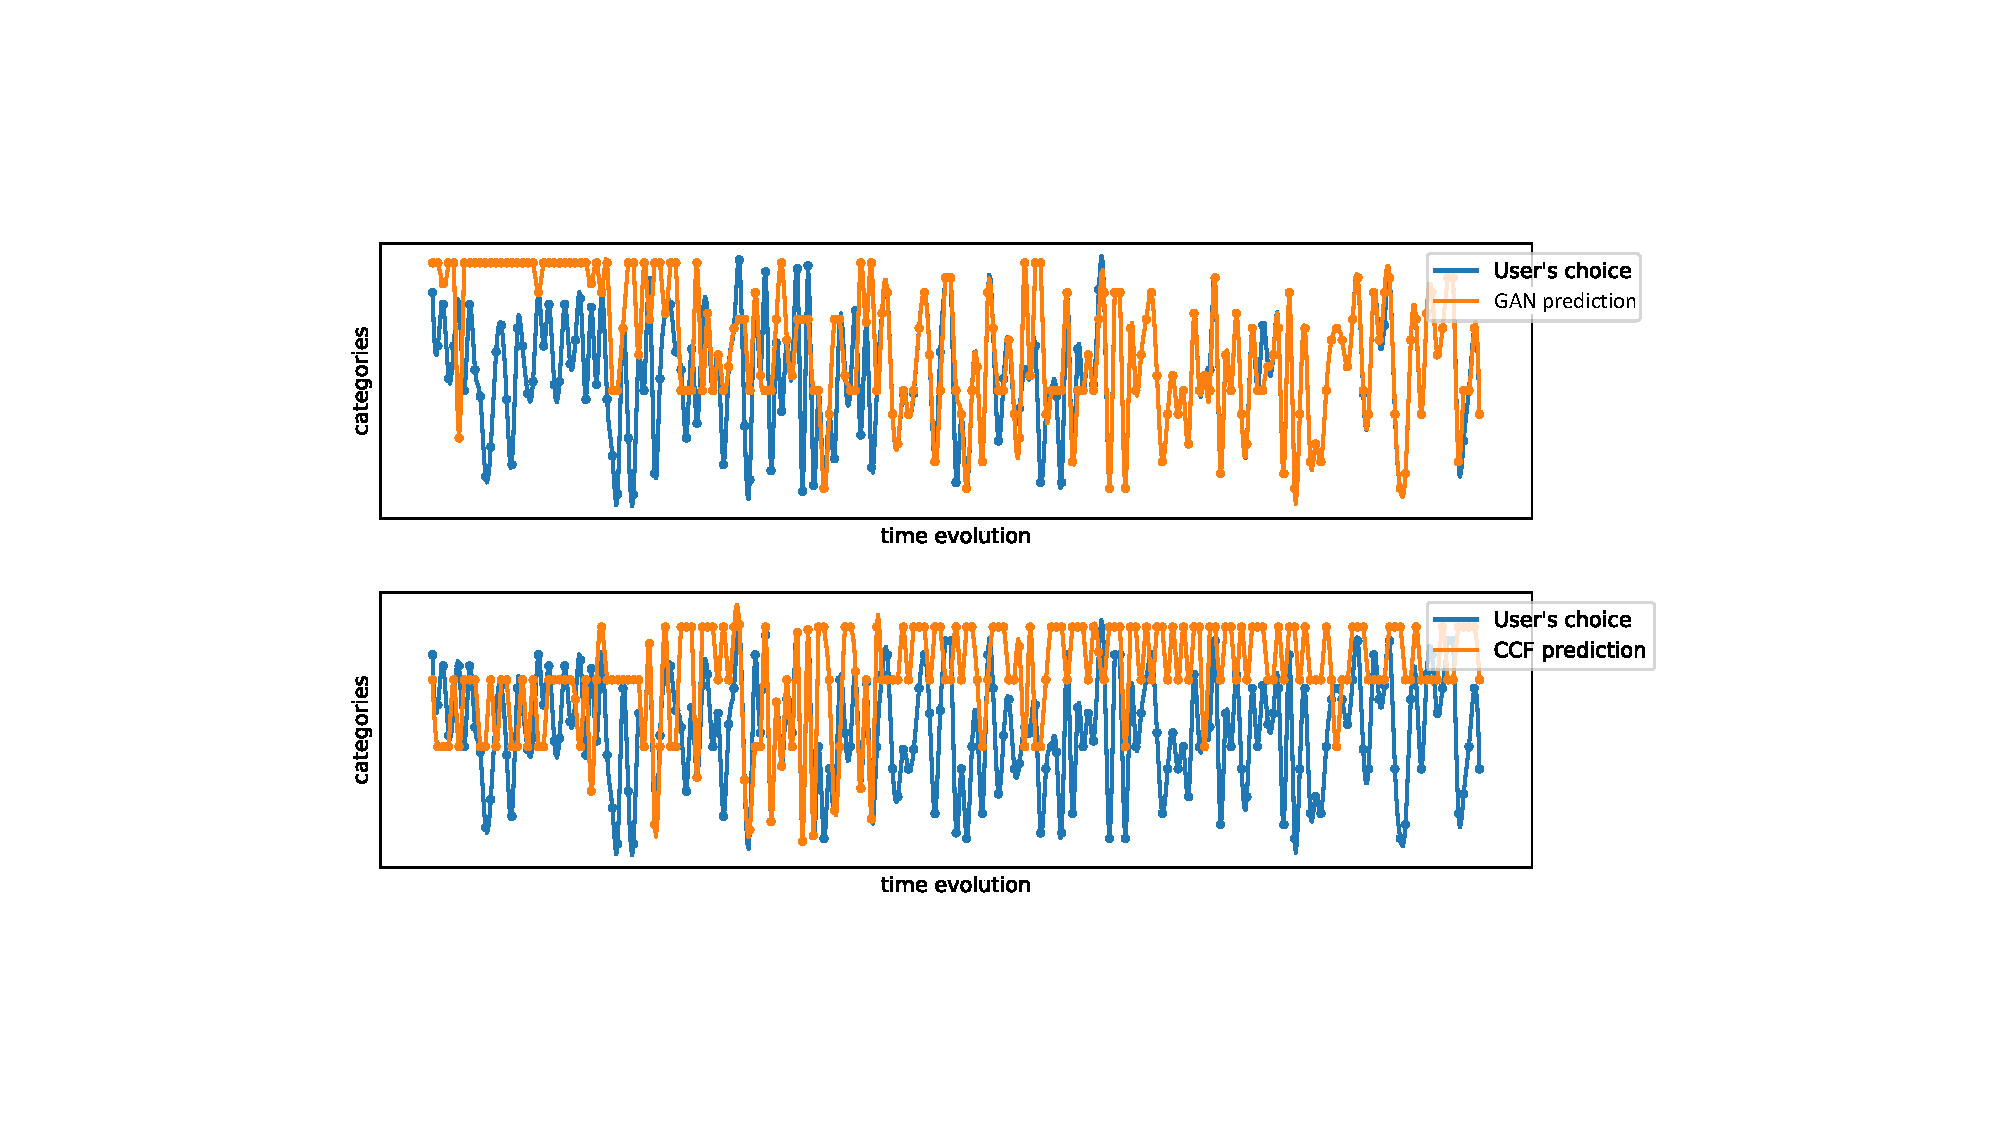
\includegraphics[width=\textwidth]{user10_new}
  \end{minipage}\hfill
  \begin{minipage}[c]{0.4\textwidth}
    \centering
    \caption{\small Comparison of the true trajectory(blue) of user's choices, the simulated trajectory predicted by GAN model (orange curve in upper sub-figure) and the simulated trajectory predicted by CCF (orange curve in the lower sub-figure) for the same user. $Y$-axis represents 80 categories of movies.
    } \label{fg:traj}
  \end{minipage}
  \vspace{-3mm}
\end{figure}

\vspace{-3mm}
\subsection{Recommendation policies generated from user models}\label{sec:experiment2}
\vspace{-3mm}

With a learned user model, one can immediately derive a greedy policy to recommend $k$ items with highest estimated likelihood. In this section, we abuse the notation {\bf LR, CCF and GAN} to represent their {\bf greedy recommendation policy} in correspondence. Apart from that, we include the RL policy based on GAN model in the experiments. We employ a deep Q network to parametrize the RL policy, so we call it {\bf GAN-DQN}.
%our GAN model provides another insight for recommendation. It is inferred by GAN model that when a user makes a choice, she will refer to her previous experience on observed items. This means the previous recommendation actions taken by the system can influence the current choice of the user.  It is noteworthy that only GAN model can help to learn a RL policy, because other models do not consider users' dynamics. 

Since we cannot make real interactions with online users at this moment, we use real data from the news article online platform to fit a user model, which we then use as a test environment. To make the experimental results trustful and solid, we fit test model on a randomly sampled set of 100 users and keep this set isolated. It is noteworthy that the 20 dimensional feature vectors are user-item cross features, so this user model is learned over user-specific features. Now we regard these 100 users as test users and the fitted model as test model. Four recommendation policies(LR, CCF, GAN, GAN-DQN) will then be evaluated among test users. All of these policies are learned from a set of 2,500 users without overlapping with the test users. The performance are evaluated by two metrics: {(1) \bf Cumulative reward}: For each recommendation action, we can observe users' behavior and compute the \Li{\st{her}} reward $r(\vs^t,a^t)$ using the test model. 
%In reality we may not be able to know the reward value for the user, but in this experiment it is accessible from test model. However, 
It should be noted that we never use the reward of test users when we train the policy. The policy is only learned on training set. The numbers shown in table~\ref{tb:policy_compare2} is the cumulative reward averaged over time horizon first and then averaged over all users. It can be formulated as $\frac{1}{100}\sum_{u=1}^{100} \frac{1}{T}\sum_{t=1}^T r^t_u$, where $r^t_u$ is the reward received by at time $t$. (2) {\bf CTR(click through rate)}: it is the ratio of the number of clicks the system receives and the number of steps it is run. This information is not only accessible in our experiment but also in practice. The value displayed in table~\ref{tb:policy_compare2} is also averaged over 100 test users.

Three sets of experiments are conducted and the results are summarized in table~\ref{tb:policy_compare2}. Since users' behavior is not deterministic, each policy is evaluated repeatedly for 50 times on test users. There are several observations: (1) Greedy policy built on GAN model is significantly better than the policies built on other models. (2) RL policy learned from GAN is better than the greedy policy. (3) Although DQN is trained to optimize the cumulative reward, it can be seen from the results that by optimizing users' reward, the recommendation system also achieves a higher click through rate.

\begin{table}[ht!]
\vspace{-1mm}
\begin{center}
    \caption{{\small Results of recommendation performances based on different user models.}}
\label{tb:policy_compare2}
\vspace{-3mm}
\resizebox{\textwidth}{!}{\begin{tabular}{l|ll|ll|ll}
\hline
\multicolumn{1}{c}{$ $}&\multicolumn{2}{|c|}{$k=2$}&\multicolumn{2}{c|}{$k=3$}&\multicolumn{2}{c}{$k=5$}\\
 \hline
model  &\multicolumn{1}{c}{reward} &\multicolumn{1}{c|}{{\footnotesize CTR}}&\multicolumn{1}{c}{reward} &\multicolumn{1}{c|}{{\footnotesize CTR}}&\multicolumn{1}{c}{reward} &\multicolumn{1}{c}{{\footnotesize CTR}}
\\ \hline
{\small LR} &  11.93($\pm$0.27) &  0.38($\pm$0.008)& 14.55($\pm$0.24) & 0.46($\pm$0.007)& 15.40($\pm$0.23)& 0.49($\pm$0.008) \\
{\small CCF} &  19.13($\pm$0.24) & 0.58($\pm$0.007)&  21.83($\pm$0.25) & 0.67($\pm$0.008)& 22.78($\pm$0.23)& 0.70($\pm$0.007)\\
{\small GAN} & 21.57($\pm$0.40) &  0.65($\pm$0.012)& 23.67($\pm$0.44)  & 0.72($\pm$0.013) & 24.35($\pm$0.42) & 0.74($\pm$0.012)\\
{\small GAN}{\scriptsize-GDQN} & { }($\pm$ )& { }($\pm$) &  {}($\pm$) & 
{}($\pm$) & {\bf 25.36}($\pm$0.30) & {\bf 0.77}($\pm$0.009)\\
{\small GAN}{\scriptsize-CDQN} & {\bf 22.76}($\pm$0.21)& {\bf 0.69}($\pm$0.007) &  {\bf 24.05}($\pm$0.26) & {\bf 0.74}($\pm$0.008) & {\bf 25.36}($\pm$0.30) & {\bf 0.77}($\pm$0.009)\\
\hline
\end{tabular}}
\end{center}
\vspace{-3mm}
\end{table}

Since table~\ref{tb:policy_compare2} only shows average value taken over all test users, we compare the policies in user level in figure~\ref{fg:policy_compare_rwd}. 
%In each sub-figure, red curve represents GAN-DQN policy and blue curve represents the other. 
GAN-DQN policy contributes higher averaged cumulative reward for most users. A similar figure which compares the click rate is attached in Appendix~\ref{app:experiment}.

\begin{figure}[ht!]
\vspace{-1mm}
\centering
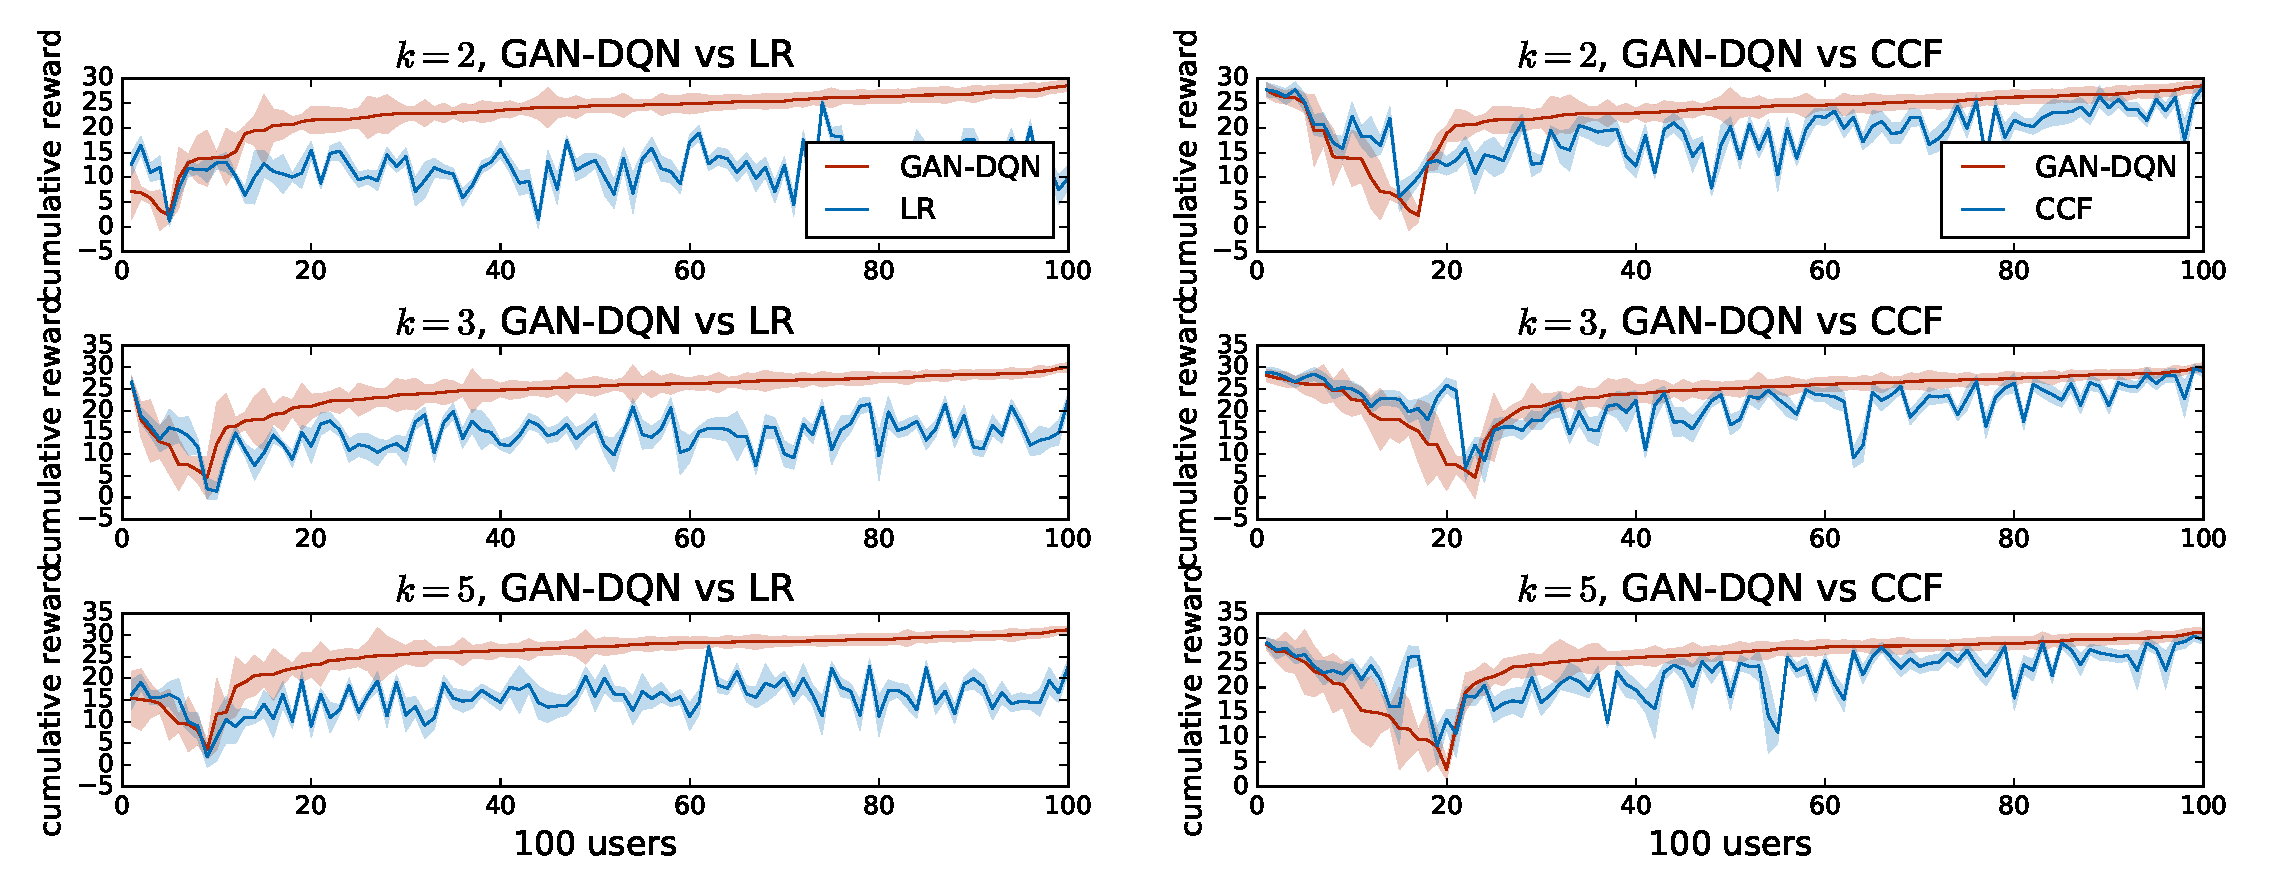
\includegraphics[width=\textwidth]{policy_compare1}	
\vspace{-5mm}
\caption{\small Cumulative rewards among 100 users under the recommendation policies based on different user models. The experiments are repeated for 50 times and standard deviation is plotted as the shaded area.}
\label{fg:policy_compare_rwd}
\vspace{-3mm}
\end{figure}

\vspace{-3mm}
\subsection{User model assisted online adaptive policies}\label{sec:experiment3}
\vspace{-3mm}

Former results in section~\ref{sec:experiment1} and \ref{sec:experiment2} have demonstrated that GAN is a better user model and its recommendation policy can achieve higher CTR compared to other user models. A question may arise as what if the recommender does not make any assumption on users and why the user model would be useful. In this section, we demonstrate by experiments how in general the user model helps recommendation polices capture users' interest faster and better. The RL policy assisted by GAN user model is compared with other policies that are learned from and adapted to online users: (1) {\bf CDQN with GAN}: cascaded deep Q-learning where the function $Q$ interacts with the learned GAN user model before it is adapted to online users. (2) {\bf CDQN without GAN}: cascaded deep Q-learning without pre-trained by the GAN model. It interacts with and adapts to online users directly. (3) {\bf LinUCB}: a classic contextual bandit algorithm which assumes adversarial user behavior. We choose its stronger version - LinUCB with hybrid linear models~\citep{LiChuLanSch10} - to compare with.

The experiment setting is similar to section~\ref{sec:experiment2}. All policies are evaluated on a separated set of 100 users associated with a test model. 
%We need to emphasize that the GAN model which assists the CDQN policy is learned from a training set of users without overlapping test users. It is different from the test model which fits the 100 test users. 
Three sets of results corresponding to different sizes of display set are plotted in figure~\ref{fg:experiment3}. It shows how the CTR increases as each policy interacts with and adapts to 100 users over time. In fact, the performances of users' cumulative reward according to different policies are also similar, for which we attach the figure in Appendix~\ref{app:exp_policy3}.

\begin{figure}[htbp]
\vspace{-4mm}
    \centering
    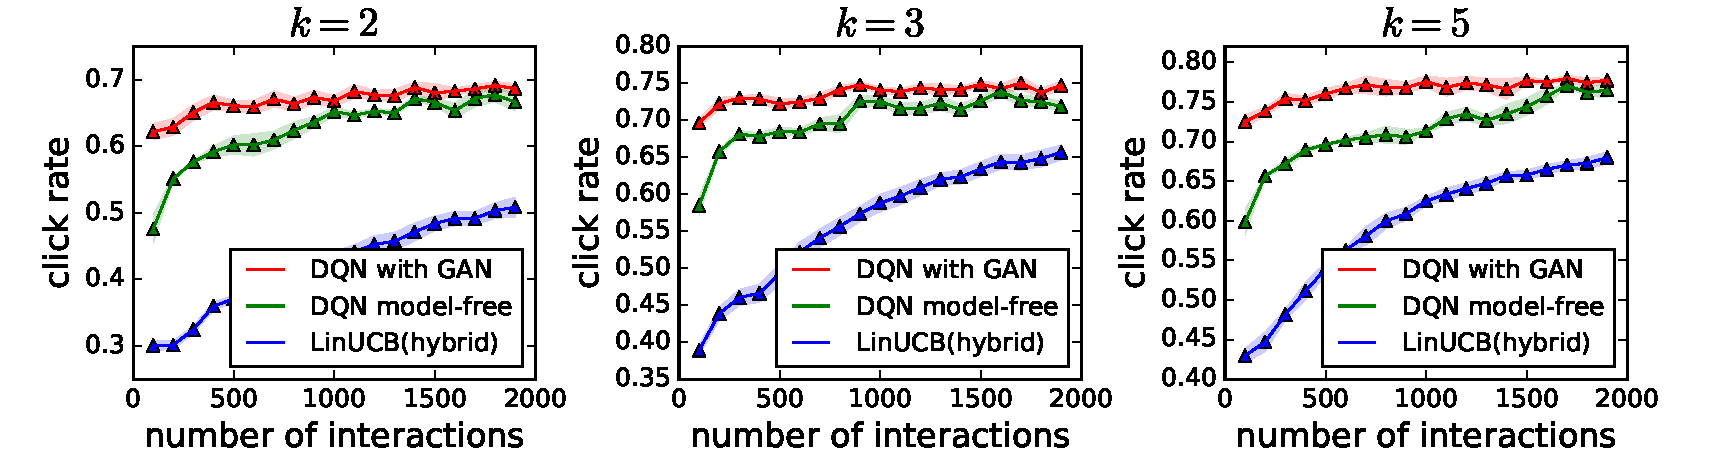
\includegraphics[width=0.95\textwidth]{Figs/policy_compare3_new.pdf}
    \vspace{-5mm}
\caption{\small Comparison of the averaged click rate among 100 users under different adaptive recommendation policies. $X$-axis represents how many times the recommender interacts with online users. Here the recommender interact with 100 users each time, so each interaction represents 100 online data points. $Y$-axis is the click rate. Each point $(x,y)$ in this figure means a click rate $y$ is achieved after $x$ many times of interactions with the users. \Li{suggest using different line type to make this figure more clear} }
\label{fg:experiment3}
\vspace{-3mm}
\end{figure}

It can be easily seen from figure~\ref{fg:experiment3} that the CDQN policy pre-trained over a GAN user model can achieve a better initial status even when it is applied to a new set of users. It can then adapt to online users fast without wasting too many trails or possibly losing the users. Without the user model, CDQN can also adapt to the users during its interaction with them. However, it takes around 1,000 iterations (i.e., 100,000 interactive data points) to achieve similar performance as the CDQN policy assisted by GAN user model. LinUCB(hybrid) is also capturing users' interest during its interaction with users, but similarly, it takes too many interactions. In Appendix~\ref{app:exp_policy3}, another figure is attached to compare the cumulative reward received by the user instead of click rate. Generally speaking, GAN user model provides a dynamic environment for RL policies to interact with to help the recommendation policy achieve a more satisfying status before applying to online users. 

\vspace{-3mm}
\section{Conclusion and Future Work}
\vspace{-3mm}

 In this paper, we propose a novel model-based reinforcement learning framework for recommendation systems, where we developed a generative adversarial network to imitate user behavior dynamics and learn her reward function. Using this user model as the simulation environment, we develop a novel DQN algorithm to obtain a combinatorial recommendation policy which can handle a large number of candidate items efficiently. Although we have try very hard to make our experiments realistic, and the experiments show clear benefits of our current method in offline and realistic simulation setting, an even stronger results could be obtained via online experimentation and A/B testing. Such experiments will be left as our future study. 

\newpage
\bibliographystyle{iclr2019_conference}
\bibliography{bibfile.bib}

\newpage

\appendix
\section{Lemma}\label{app:proof}
\subsection{Proof of lemma~\ref{lm:lemma1}} 
\primelemma*
\begin{proof}
First, recall the problem defined in~\eqref{eq:max}:
\[
\phi^*(\vs^t,\gA^t) = \arg\max_{\phi \in \Delta^{k-1}} \E_{\phi} \left[r(\vs^t, a^t) \right] -\frac{1}{\eta}\E_{\phi}[R(\phi)].
\]
Denote $\phi^t = \phi(\vs^t,\gA^t)$. Since $\phi$ can be an arbitrary mapping (i.e., $\phi$ is not limited in a specific parameter space), $\phi^t$ can be an arbitrary vector in $\Delta^{k-1}$. Recall the notation $\gA^t = \{a_1,\cdots, a_k\}$. Then the expectation taken over random variable $a^t\in \gA^t$ can be written as
\begin{equation}\label{eq:lm1_1}
     \E_{\phi} \left[r(\vs^t, a^t) \right] -\frac{1}{\eta}\E_{\phi}[R(\phi)] =\sum_{i=1}^k \phi_i^tr(\vs^t, a_i) -\frac{1}{\eta} \sum_{i=1}^k \phi_i^t \log \phi_i^t.
\end{equation}
By simple computation, the optimal vector $\phi^{t*}\in \Delta^{k-1}$ which maximizes~\eqref{eq:lm1_1} is
\begin{equation}\label{eq:lm1_2}
    \phi_i^{t*} =\dfrac{\exp(\eta r(\vs^t, a_i))}{\sum_{j=1}^{k}\exp(\eta r(\vs^t, a_j))},
\end{equation}
\Li{fix the typo in above equation.}
which is equivalent to~\eqref{eq:max}. Next, we show the equivalence of~\eqref{eq:lm1_2} to the discrete choice model interpreted by~\eqref{eq:gumbel}.

The cumulative distribution function for the Gumbel distribution is $F(\varepsilon;\alpha) = \mathbb{P}[\varepsilon \leqslant \alpha ] = e^{-e^{-\alpha}}$ and the probability density is $f(\varepsilon) = e^{-e^{-\varepsilon}}e^{-\varepsilon} $. Using the definition of the Gumbel distribution, the probability of the event $[a^t = a_i]$ where $a^t$ is defined in~\eqref{eq:gumbel} is 
\begin{align*}
    P_i :=  \mathbb{P} \Big[a^t = a_i\Big] &= \mathbb{P} \Big[ \eta r(\vs^t,a_i) +\varepsilon_i \geqslant \eta r(\vs^t,a_j) +\varepsilon_j ,  \text{ for all } i\neq j \Big]\\
    & =  \mathbb{P} \Big[\varepsilon_j \leqslant\varepsilon_i + \eta r(\vs^t,a_i)-\eta r(\vs^t,a_j),  \text{ for all } i\neq j \Big].
\end{align*}
Suppose we know the random variable $\varepsilon_i$. Then we can compute the choice probability $P_i$ conditioned on this information. Let $B_{ij} = \varepsilon_i +\eta r(\vs^t,a_i)-\eta r(\vs^t,a_j) $ and $P_{i|\mathcal{E}}$ be the conditional probability; then we have
\[
P_{i|\varepsilon_i} = \prod_{i \neq j} \mathbb{P}[\varepsilon_{j} \leqslant B_{ij}] = \prod_{i \neq j} e^{-e^{-B_{ij}}}.
\]
In fact, we only know the density of $\varepsilon_i$. Hence, using the Bayes theorem, we can express $P_i$ as
\begin{align*}
P_i & = \int_{-\infty}^{\infty} P_{i|\varepsilon_i} f(\varepsilon_i) \rd \varepsilon_i = \int_{-\infty}^{\infty} \prod_{i \neq j} e^{-e^{-B_{ij}}} f(\varepsilon_i) \rd \varepsilon_i \\
&  = \int_{-\infty}^{\infty} \prod_{j=1}^k e^{-e^{-B_{ij}}}   e^{e^{-\varepsilon_i}} e^{-e^{-\varepsilon_i}}e^{-\varepsilon_i} \rd \varepsilon_i= \int_{-\infty}^{\infty} \Big( \prod_{j=1}^k e^{-e^{-B_{ij}}} \Big)  e^{-\varepsilon_i} \rd \varepsilon_i
\end{align*}
Now, let us look at the product itself.
\begin{align*}
\prod_{j=1}^k e^{-e^{-B_{ij}}} & = \exp\Big( -\sum_{j=1}^k e^{-B_{ij}}\Big) \\
& = \exp \Big( - e^{-\varepsilon_i }\sum_{j=1}^k e^{- (\eta r(\vs^t,a_i)-\eta r(\vs^t,a_j) )} \Big)
\end{align*}
Hence 
\[
P_i = \int_{-\infty}^{\infty} \exp(-e^{-\varepsilon_i } Q ) e^{-\varepsilon_i} \rd \varepsilon_i
\]
    where $Q = \sum_{j=1}^k e^{- (\eta r(\vs^t,a_i)-\eta r(\vs^t,a_j) )}  = Z/\exp(\eta r(\vs^t,a_i) )$. 

Next, we make a change of variable $y = e^{-\varepsilon_i}$. The Jacobian of the inverse transform is $J = \frac{\rd \varepsilon_i}{\rd y} = -\frac{1}{y}$. Since $y>0$, the absolute of Jacobian is $|J| = \frac{1}{y}$. Therefore, 
\begin{align*}
P_i & = \int_{0}^{\infty} \exp(-Q y) y |J| \rd y=\int_{0}^{\infty} \exp(-Q y)\rd y	\\
& = \frac{1}{Q} = \frac{1}{\exp(-\eta r(\vs^t,a_i)) \sum_j \exp(\eta r(\vs^t,a_j))}\\
& = \dfrac{\exp(\eta r(\vs^t, a_i)}{\sum_{j=1}^k \exp(\eta r(\vs^t, a_j))}.
\end{align*}
\end{proof}
\subsection{Proof of lemma~\ref{lm2:mle}} 
\secondlemma*
\begin{proof}This lemma is a straight forward result of lemma~\ref{lm:lemma1}.
First, recall the problem defined in~\eqref{eq:std-minmax}:
\[
\min_{\theta \in \Theta} \left(\max_{\phi\in \Phi}  \E_{\phi} \left[\sum_{t=1}^Tr_{\theta}(\vs^t_{true}, a^t) -\frac{1}{\eta}R(\phi)\right]\right)-\sum_{t=1}^T r_{\theta}(\vs^t_{true}, a^t_{true})
	\]
We make a assumption that there is no repeated pair $(\vs^t_{true}, a^t)$ in~\eqref{eq:std-minmax}. This is a very soft assumption because $\vs^t_{true}$ is updated overtime, and $a^t$ is in fact representing its feature vector $\vf^t_{a^t}$, which is in space $\mathbb{R}^d$. With this assumption, we can let $\phi$ map each pair $(\vs^t_{true}, a^t)$ to the optimal vector $\phi^{t*}$  which maximize $r_{\theta}(\vs^t_{true}, a^t) -\frac{1}{\eta}R(\phi^t)$ since there is no repeated pair. Using~\eqref{eq:lm1_2}, we have
\begin{align*}
&\max_{\phi\in \Phi}  \E_{\phi} \left[\sum_{t=1}^Tr_{\theta}(\vs^t_{true}, a^t) -\frac{1}{\eta}R(\phi)\right] = \max_{\phi\in \Phi} \sum_{t=1}^T \E_{\phi} \left[r_{\theta}(\vs^t_{true}, a^t) -\frac{1}{\eta}R(\phi)\right] \\
    =& \sum_{t=1}^T\left(   \sum_{i=1}^k \phi_i^{t*}r(\vs^t, a_i) -\frac{1}{\eta} \sum_{i=1}^k \phi_i^{t*} \log \phi_i^{t*} \right)=\sum_{t=1}^T\frac{1}{\eta}\log\Big(\sum_{i=1}^k \exp(\eta r_{\theta}(\vs^t_{true}, a_i))\Big).
\end{align*}~\eqref{eq:std-minmax} can then be written as
\[
\min_{\theta\in\Theta}\sum_{t=1}^T\frac{1}{\eta}\log\Big(\sum_{i=1}^k \exp(\eta r_{\theta}(\vs^t_{true}, a_i))\Big) - \sum_{t=1}^T r_{\theta}(\vs^t_{true}, a^t_{true}),
\]
which is the negative log-likelihood function and is equivalent to lemma~\ref{lm2:mle}.
\end{proof}

\section{Alogrithm box}\label{app:algo}

\begin{algorithm}[ht!]
\caption{Cascading deep Q-learning (CDQN) with Experience Replay}
\label{alg:dqn}
\begin{algorithmic}[1]
\State Initialize replay memory $\gM$ to capacity $N$ 
\State Initialize parameter $\Theta_j$ of $\widehat{Q^j}$ with random weights for each $1\leq j\leq k$
\For{iteration $i=1$ to $L$}
	\State Sample a batch of users $\gU$ from training set
	\State Initialize the states ${\vs}^0$ to a zero vector for each $u\in \gU$
	\For{$t=1$ to $T$}
	    \For{each user $u\in \gU$ simultaneously}
	        \State With probability $\epsilon$ select a random subset $\gA^t$ of size $k$\label{line:epsilon-greedy}
		    \State Otherwise, $\displaystyle \gA^t =
	\textsc{argmax\_Q}(\vs_u^t, \gI^t, \Theta_1,\cdots,\Theta_k)$\label{line:argmax}
 		    \State Recommend $\gA^t$ to user $u$, observe user action $a^t\sim\phi(\vs^t,\gA^t)$ and update user state $\vs^{t+1}$
		    \State Add tuple $\big(\vs^t, \gA^t, r(\vs^t, a^t), \vs^{t+1}\big)$ to $\gM$\label{line:exp_replay1}
		\EndFor
		\State Sample random minibatch $B\overset{\text{iid.}}{\sim}\gM$\label{line:exp_replay2}
		\State For each $j$, update $\Theta_j$ by SGD over the loss $\big(y- \widehat{Q^j}(\vs^t, A^t_{1:j}; \Theta_j)\big)^2$ for $B$\label{line:exp_replay3}
	\EndFor
\EndFor
\State \Return $\Theta_1,\cdots,\Theta_k$
\end{algorithmic}
\end{algorithm}

\Li{the notation $A^t_{1:j}$ is not defined?}

\section{Dataset description}\label{app:dataset}
{\bf (1) MovieLens public dataset} contains large amounts of movie ratings collected from their website. We randomly sample 1,000 active users from this dataset. On average, each of these active users rated more than 500 movies (including short films), so we assume they rated almost every movie that they watched and thus equate their rating behavior with watching behavior. MovieLens dataset is the most suitable public dataset for our experiments, but it is still not perfect. In fact, none of the public datasets provides the context in which a user's choice is made. Thus, we simulate this missing information in a reasonable way. For each movie watched(rated) on the date $d$, we collect a list of movies released within a month before that day $d$. On average, movies run for about four weeks in theater. Even though we don't know the actual context of user's choice, at least the user decided to watch the rated movie instead of other movies in theater. Besides, we control the maximal size of each displayed set by 40. {\bf Features:} In MovieLens dataset, only titles and IDs of the movies are given, so we collect detailed movie information from Internet Movie Database(IMDB). Categorical features as encoded as sparse vectors and descriptive features are encoded as dense vectors. The combination of such two types of vectors produces 722 dimensional raw feature vectors. To further reduce dimensionality, we use logistic regression to fit a wide\&deep networks~\citep{ChengKocHarmsen16} and use the learned input and hidden layers to reduce the feature to 10 dimension.

{\bf (2) An online news article recommendation dataset from Ant Financial} is anonymously collected from Ant Financial news article online platform. It consists of 50,000 users' clicks and impression logs for one month, involving dozens of thousands of news. It is a time-stamped dataset which contains user features, news article features and the context where the user clicks the articles. The size of the display set is not fixed, since a user can browse the news article platform as she likes. On average a display set contains 5 new articles, but it actually various from 2 to 10.  {\bf Features:} The news article raw features are approximately of dimension 100 million because it summarizes the key words in the article. Apparently it is too expensive to use these raw features in practice. The features we use in the experiments are 20 dimensional dense vector embedding produced from the raw feature by wide\&deep networks. 
% ensembling the results of multiple score functions whose structures are comparatively simple. 
The reduced 20 dimensional features are widely used in this online platform and revealed to be effective in practice.

\section{More figures for experimental results}\label{app:experiment}
\subsection{Figures for section~\ref{sec:experiment1}}\label{app:exp_usermodel}
An interesting comparison is shown in Figure~\ref{fg:traj} and more similar figures are provided here. The blue curve is the trajectory of a user's actual choices of movies over time. The orange curves are simulated trajectories predicted by GAN and CCF, respectively. Similar to what we conclude in section~\ref{sec:experiment1}, these figures reveal the good performances of GAN user model in terms of capturing the evolution of users' interest. 
\begin{figure}[htbp]
  \begin{minipage}[c]{0.47\textwidth}
    \centering
    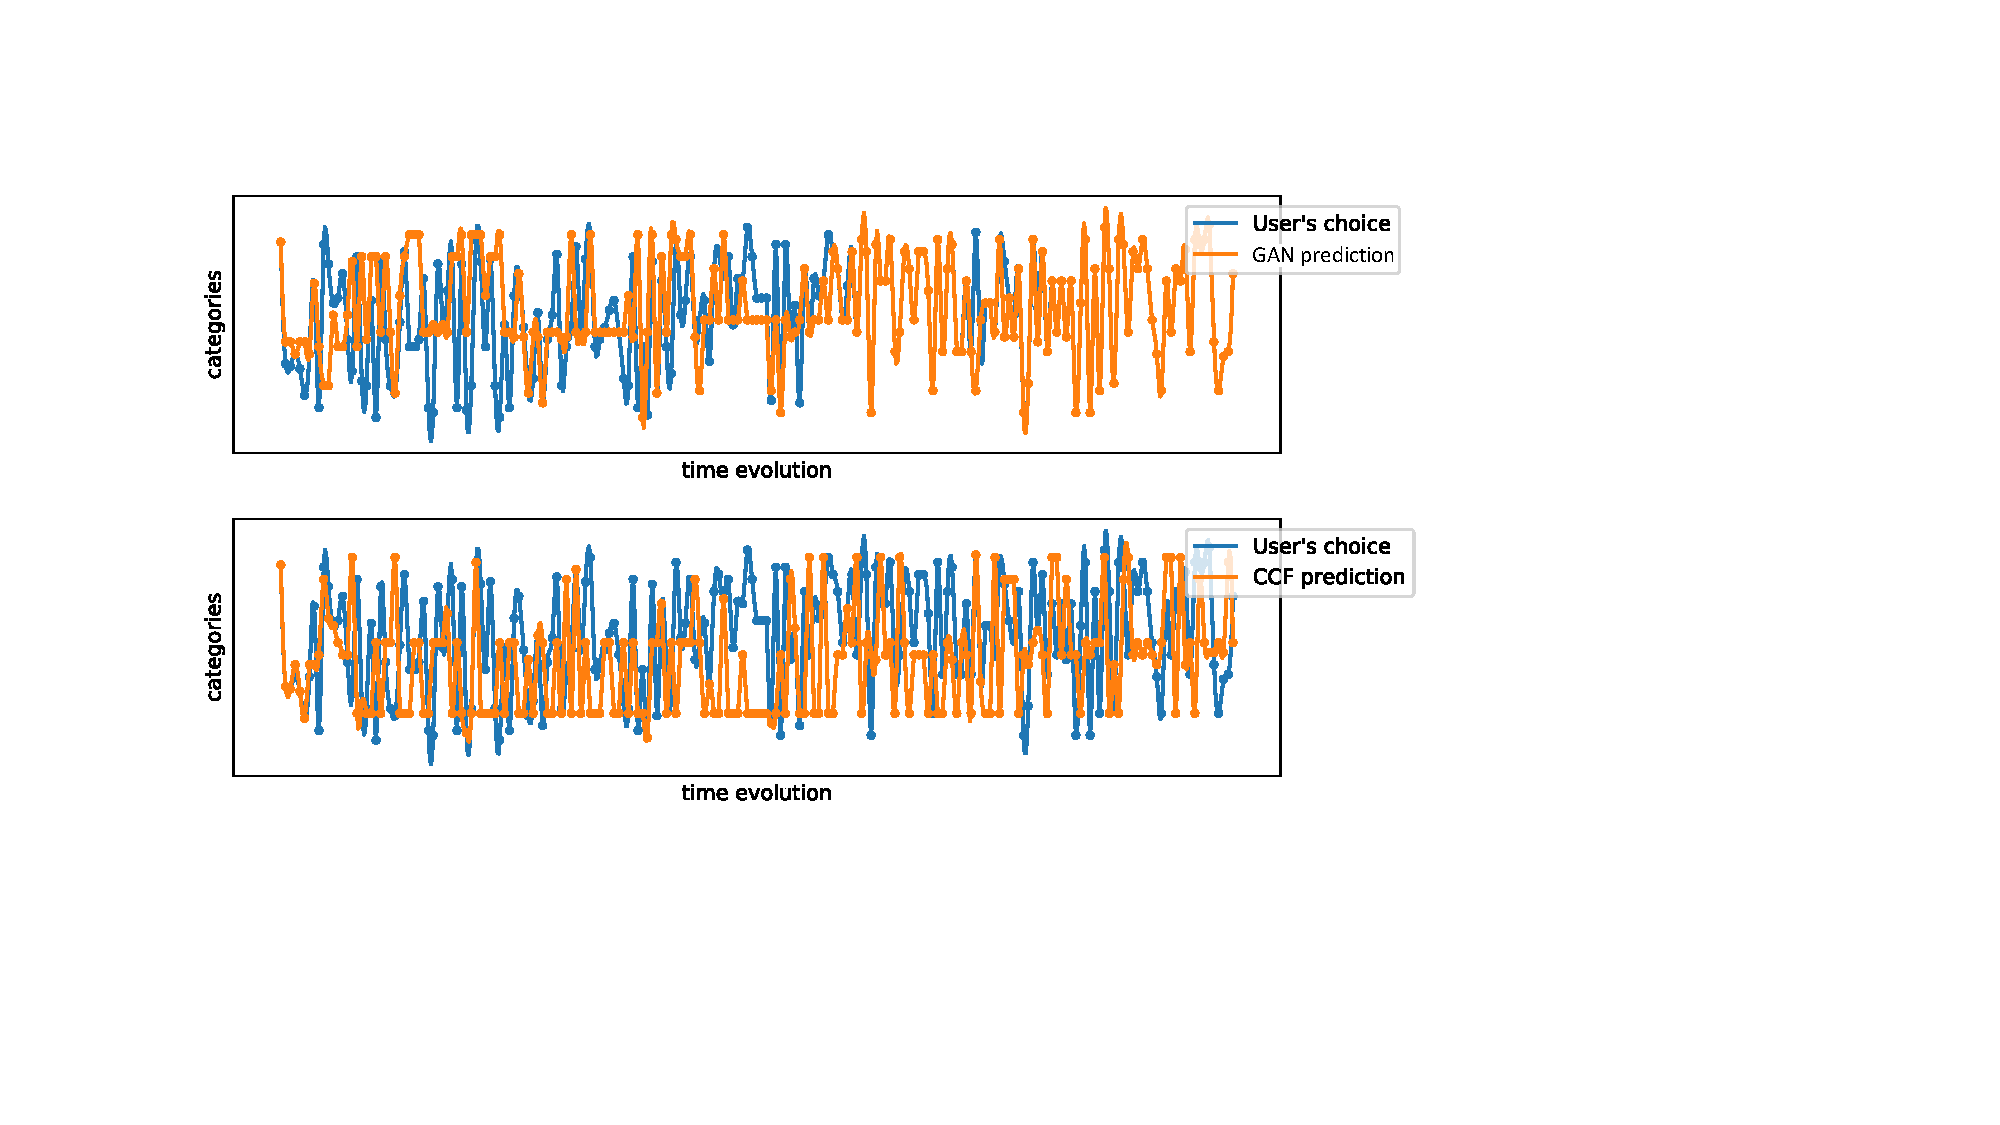
\includegraphics[width=\textwidth]{user18_new}
  \end{minipage}\hfill
  \begin{minipage}[c]{0.52\textwidth}
    \centering
        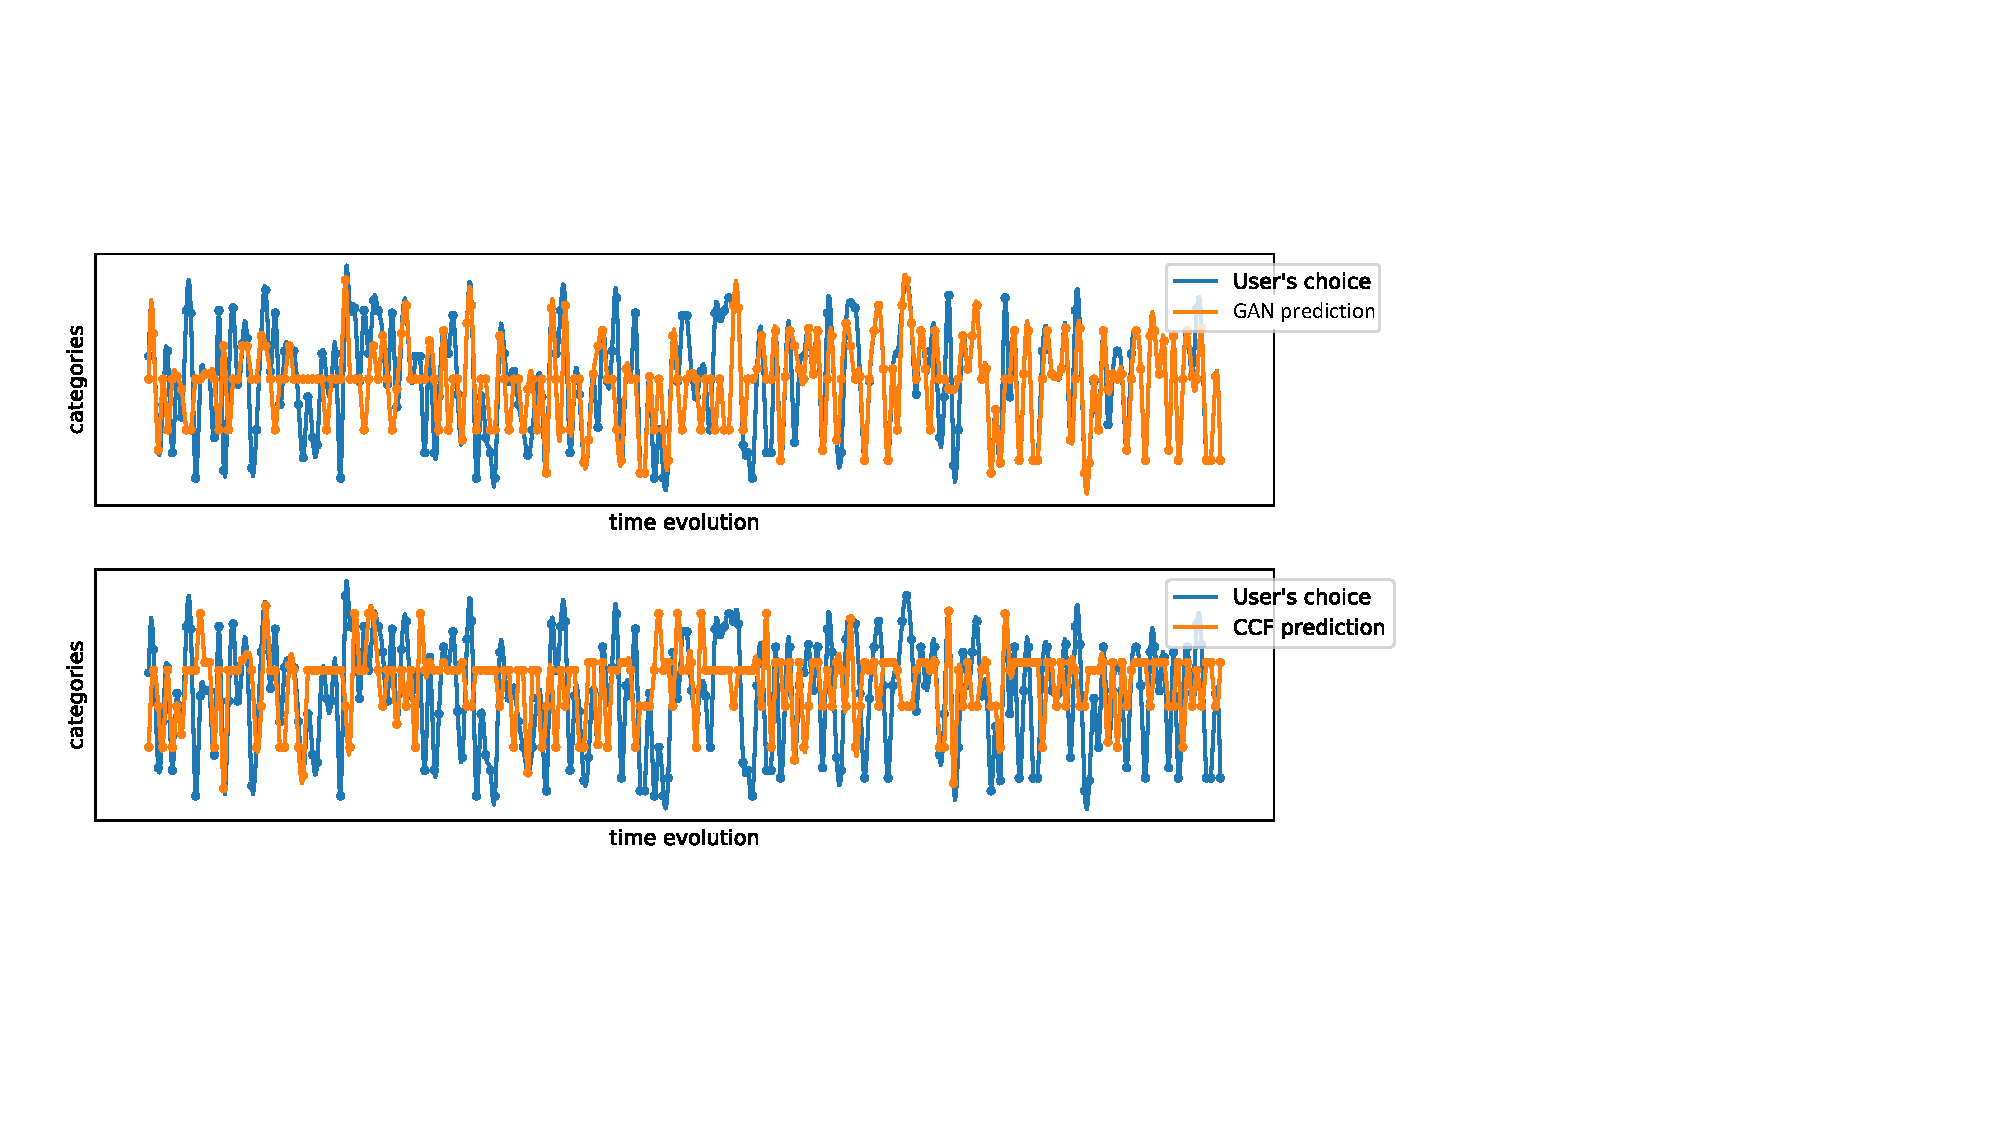
\includegraphics[width=\textwidth]{user19_new}
  \end{minipage}
  \caption{\small Two more examples: comparison of the true trajectory(blue) of user's choices, the simulated trajectory predicted by GAN model (orange curve in upper sub-figure) and the simulated trajectory predicted by CCF (orange curve in the lower sub-figure) for the same user. $Y$-axis represents 80 categories of movies.
    }
\end{figure}


\subsection{Figures for section~\ref{sec:experiment2}}\label{app:exp_policy2}
 We demonstrate the policy performance in user level in figure~\ref{fg:policy_compare_rwd} by comparing the cumulative reward. Here we attach the figure which compares the click rate. In each sub-figure, red curve represents GAN-DQN policy and blue curve represents the other. GAN-DQN policy contributes higher averaged click rate for most users.
\begin{figure}[ht!]
\centering
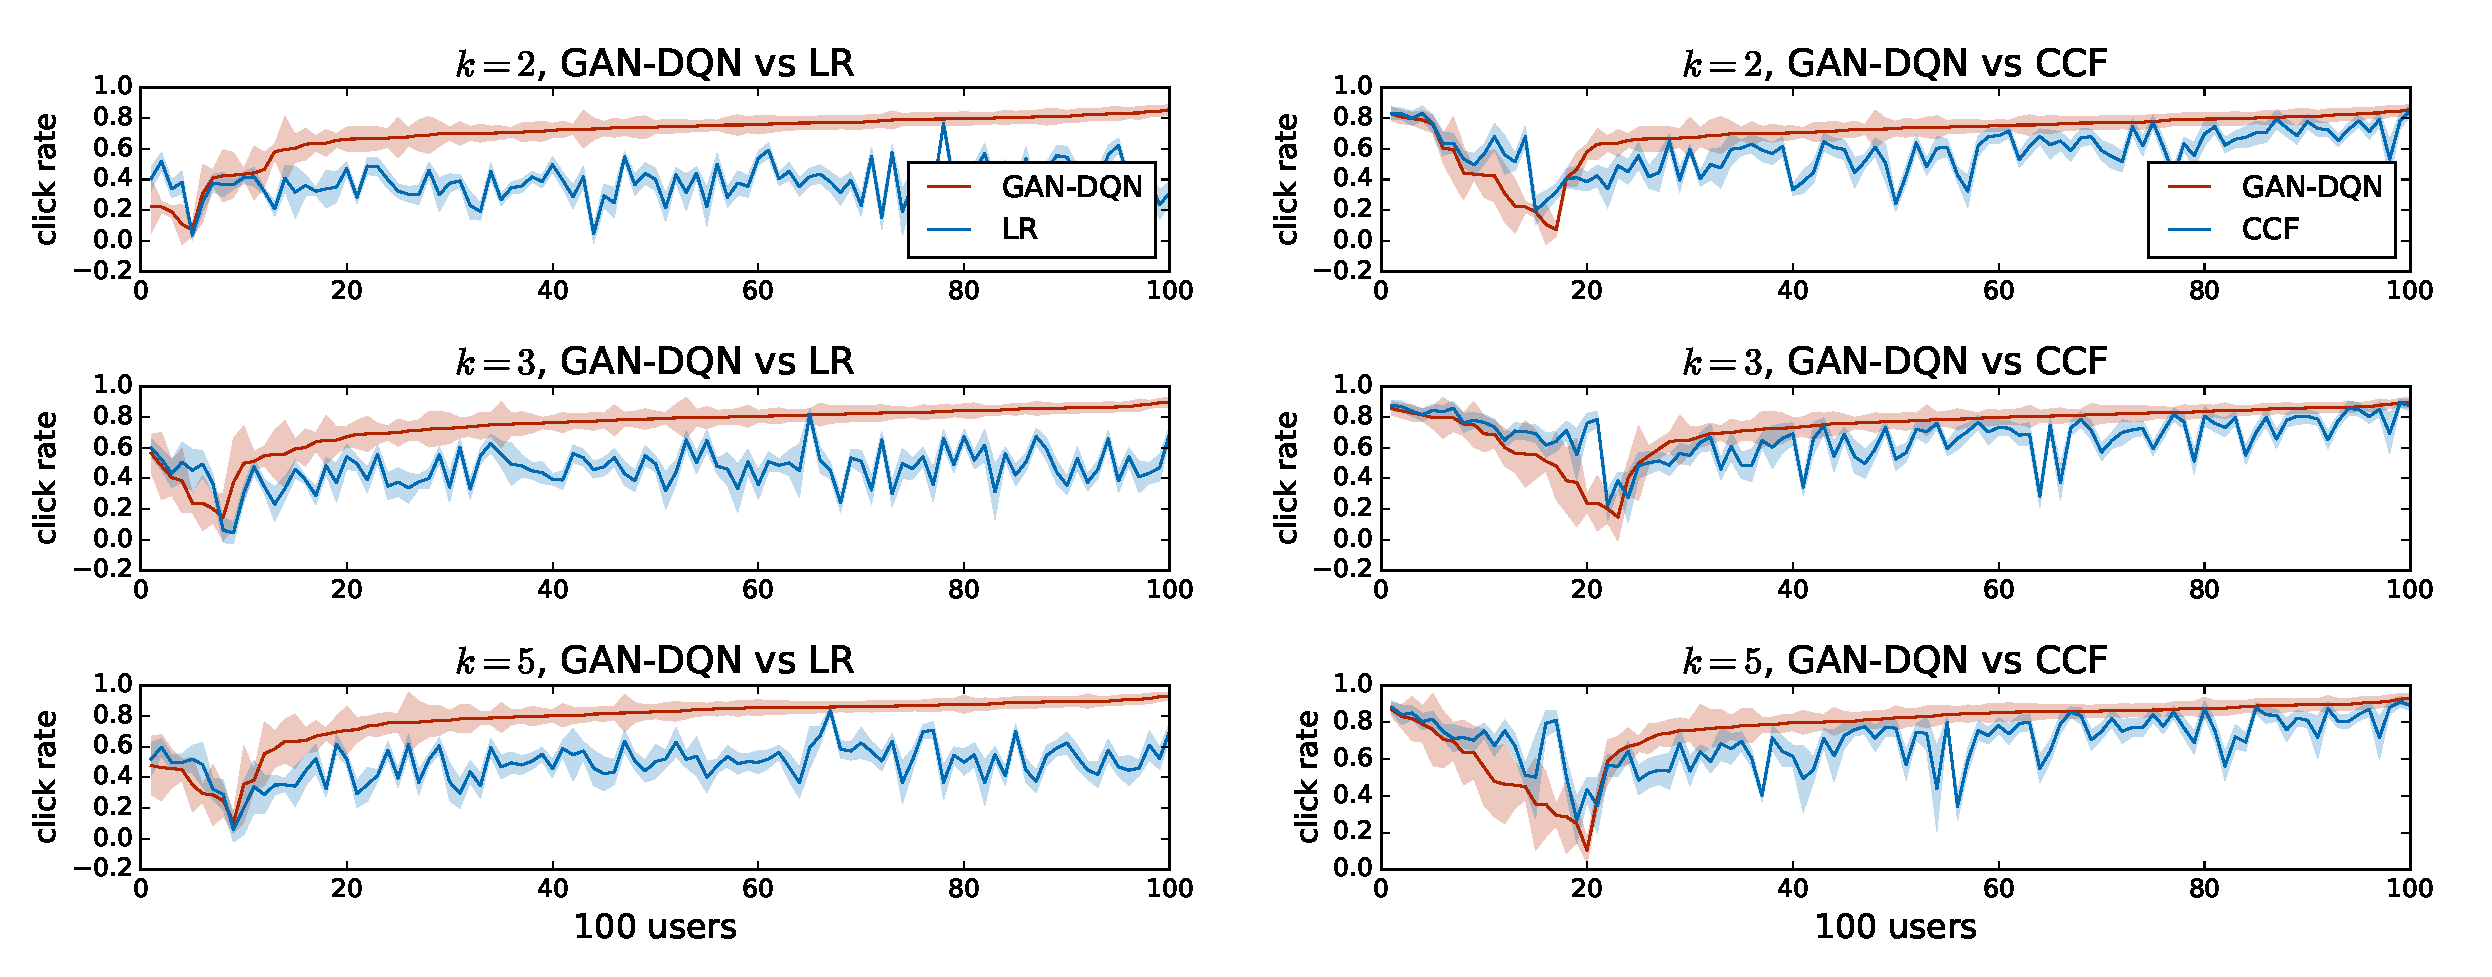
\includegraphics[width=\textwidth]{policy_compare1_CTR.pdf}	
\caption{\small Comparison of click rates among 100 users under the recommendation policies based on different user models. In each figure, red curve represents GAN-DQN policy and blue curve represents the other. The experiments are repeated for 50 times and standard deviation is plotted as the shaded area. This figure is similar to figure~\ref{fg:policy_compare_rwd}, except that it plots the value of click rates instead of user's cumulative rewards.}
\end{figure}

\subsection{Figures for section~\ref{sec:experiment3}}\label{app:exp_policy3}
This figure shows three sets of results corresponding to different sizes of display set. It reveals how users' cumulative reward(averaged over 100 users) increases as each policy interacts with and adapts to 100 users over time. It can be easily that the CDQN policy pre-trained over a GAN user model can adapt to online users much faster then other model-free policies and can reduce the risk of losing the user at the beginning. The experiment setting is similar to section~\ref{sec:experiment2}. All policies are evaluated on a separated set of 100 users associated with a test model. We need to emphasize that the GAN model which assists the CDQN policy is learned from a training set of users without overlapping test users. It is different from the test model which fits the 100 test users. 
\begin{figure}[htbp]
    \centering
    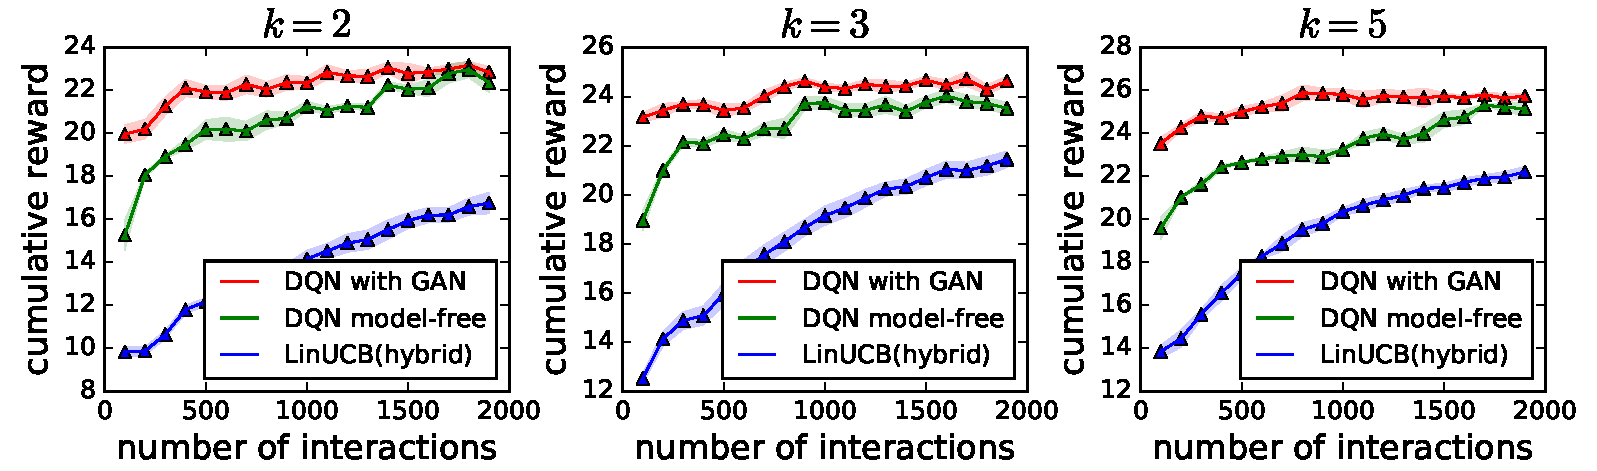
\includegraphics[width=0.85\textwidth]{Figs/policy_compare3_rwd.pdf}
\caption{\small Comparison of the averaged cumulative reward among 100 users under different adaptive recommendation policies. $X$-axis represents how many times the recommender interacts with online users. Here the recommender interact with 100 users each time, so in fact each interaction represents 100 online data points. $Y$-axis is the click rate. Each point $(x,y)$ in this figure means a click rate $y$ is achieved after $x$ many times of interactions with the users. }
\end{figure}
\end{document}
